\documentclass{article}
\usepackage{graphicx} 
\usepackage{geometry}
\geometry{
    a4paper,
    total={170mm,257mm},
    left=20mm,
    top=20mm,
}
\usepackage[hidelinks]{hyperref}
\usepackage{xcolor}
\usepackage{natbib}
\bibliographystyle{apalike}
\usepackage{tikz}
\usetikzlibrary{mindmap, trees}
\usepackage{siunitx}
\usepackage{xcolor}
\usepackage{rotating}
\usepackage{threeparttable}
\usepackage{pdflscape}
\usepackage{parskip}
\usepackage{subcaption}
\usepackage{tabularx}
\usepackage{booktabs}
\usepackage{authblk}
\usepackage{longtable}
\usepackage{ragged2e}
\usepackage{multirow}
\usepackage{makecell}

\newcolumntype{b}{X}
\newcolumntype{s}{>{\hsize=.5\hsize}X}
\newcolumntype{m}{>{\hsize=.75\hsize}X}

\renewcommand{\arraystretch}{1.3}

\title{A new sequential accident model to classify single-cyclist crashes based on known mechanisms explained through physics}


\author[1]{Benjamín E. González T.}
\author[1]{Ajay Seth}
\author[1]{Alfred Schouten}
\author[1]{Jason K. Moore}
%
\affil[1]{\footnotesize{Department of Biomechanical Engineering, Delft University of Technology}}
\date{}

\begin{document}

% \clearpage

\maketitle


% ----- Jason comments -----
% - You have an elaborate classification in Figure 3 (the big flow chart) but the later part of the paper seems to have people only classify bicycle motion and label in 3 categories. I miss what happens to everything else in figure 3.
% - If the questionnaire results are included, the quality needs to be raised to meet standards of survey experiments. Otherwise you can only say something like "I had 10 colleagues review my classification and they all agreed to 90\%." or something similar. I also have a worry in the design, which may have implicitly coached your subjects to give you the answers that match your opinion.
% - I'd like to see, via figures and/or tables, how your classification relates to prior work. Is it possible to show how you morphed what you saw into what you have?
% - It seems your central claim at the end is that your classification captures all falls and few are put into "other". But I list several falls that I don't see fitting into the 3 categories you have. I feel that the 3 are too few. Maybe they are only three and so broad each that you can imagine each fall fitting into them. But is that ultimately helpful? The extreme would be 1 category "this is a fall" or "this is not a fall". We can all probably bin everything into those two. Of course, it is more difficult to bin things the more fine grain your categories are. So is the fact that you have no "other" items because you've made the categories too general? versus it being details and all encompassing?
% - What do you see as the implications of your new method? How will people use this? Will it be useful? Will you use it? If so, why? If you spend the time to create this, you want people to use it so it is worth thinking about whether you are creating something that can have impact and explain how it might be impactful in the paper. Think about what you want to accomplish by the end of your PhD, will this classification play an important role in achieving that?
% - Can you demonstrate how Figure 3 would be fully applied to the characterization of a crash? This would be very valuable as it can demonstrate the power of the entire classification.
% ----- -----




\small

\section*{Keywords}
%
Single-bicycle crash;
%
Crash configurations;
%
Bicycle dynamics;
%
Crash mechanisms;
%

%%


\section*{Abstract} 
%
\textbf{
Single-cyclist crashes are one of the main issues in the cycling safety field; however, the physics underlying the causes is still unclear.
%
An important constraint on the study of the dynamics of single-cyclist crashes is the lack of a classification with focus on the crash mechanisms. 
%
Therefore, the aim of the present work is to develop a single-cyclist crash classification based on bicycle dynamics.
%
To this end, existing classifications were revised to discuss the hypothesised mechanisms and causes, to be later contrasted with the theory of bicycle and motorcycle dynamics.
%
The proposed classification works under the multi-layer principle, allowing the combination of factors to respond to modern crash models' requirements.
%
The resulting classes are manoeuvre, excitation of the system, crash mechanisms and characteristic motion.
%
These classes are related by causality, where it is possible to specify root causes between layers.
%
Additionally, this work includes sub-classes for rider control, signal input, and location of the fault mechanism.
%
In this way, the proposed failure mechanisms are balance control, contact forces, load transfer, rider-bicycle joint, and tyre friction.
%
Along, the crash motions are collision ejection, pitch-over, and roll-over, which is sub-divided in three: Tip-over, Low-side, and High-side.
%
This classification serves as a base for classifying single-cyclist crashes through different disciplines and gathering as much information as possible to recreate the crash for its analysis.
}


\normalsize
\section{Introduction} \label{sec: introduction}
%
Cycling is on the rise due to the advantages of the bicycle as a commuter vehicle.
%
The low cost of transportation and maintenance, together with less pollution, healthier lifestyles and less traffic congestion, all contribute to the advantages.
%
However, cyclists are vulnerable road users who are exposed to the environment and other road users with no major protection.
%
For this reason, the severity of bicycle incidents tends to be higher than car passengers.
%%


Although the absolute number of bicycle fatalities has reduced, its share with respect to the total road casualties has increased across Europe \citep{CBS24, Eur24}.
%
From \cite{CBS24} it is known that the average of car fatalities decreased by 17\% from 2013 to 2023, while cyclist fatalities increased by 22\% in the same period.
%
Furthermore, one configuration of bicycle crashes that stands out due to its major share on statistics from the Netherlands is the Single-Cyclist Crash (SCC) \citep{Weg24}.
%
These are events where no other road user is involved, specifically, single-cyclist crashes account for 80\% of cyclist-related hospital admissions in the Netherlands \citep{Boe17}.
%
Moreover, these numbers repeat the trend in other countries: 50\% to 85\% in Finland \citep{Utr23}, 68\% in Sweden \citep{Ohl19}, \textgreater50\% in Australia \citep{Bou13}, 31\% in Belgium \citep{Van16}, and 29\% in Ireland \citep{Gil21a}.
%
It is important to note that the focus of the present work is on the occurrence of crashes; therefore, there is no discrimination between studies about injuries and fatalities.
%%



Indeed, in the Netherlands, the risk of death in single-cyclist crashes has not only remained constant, but increased up to 7\% in the period from 1996 to 2014 \citep{Sch17}. 
%
Hence, these events are a matter of interest when bicycle usage is intended to be promoted and risks need to be minimised \citep{Eur24}.
%
Furthermore, if these issues are not addressed, bicycle usage may decrease \citep{Gu19}.
%%



A key factor in the increasing share of bicycle crashes is the constant reduction of motorised vehicle crashes~\citep{Swo25}.
%
These vehicles have benefited from several driving assistance systems, such as stability control, anti-lock braking systems, and collision avoidance systems, among others \citep{Ben14}.
%
Hence, the cognitive load for the driver has been reduced, giving them a wider margin to commit mistakes without leading to a crash.
%
Contrarily, bicycles have seen minimal technological evolution throughout the years, with the exception of electric pedal assistance \citep{Kap22}.
%
Therefore, bicycle safety technology may be able to similarly reduce crash occurrences. 
%
Thus, the first step in mitigating crashes with technology is to develop a causal and mechanistic understanding of the crashes.
%%


The literature states that a crash is an interplay of three factors: vehicle, human, and environment \citep{Fel76, Zha22}.
%
From these, environmental factors, i.e. infrastructure design and interaction with other road users, have been thoroughly assessed and improved in the last decade \citep{Sch17a}.
%
Conversely, the human is known to be a strong factor \citep{Orm08}, but its role in the outcome of the event is not yet fully understood.
%
Furthermore, the role of the bicycle has not been properly assessed, since past data is not detailed enough to extract the kinematic and dynamic mechanisms.

the understanding of the dynamics of the crashes is still scarce.
%
As \cite{SWO23} states, \textit{`...whether the vehicle features of bicycles play a role in crash occurrence is hard to determine, and even if this role is determined, it is not systematically registered...'}
%
Therefore, it is necessary to understand the crash dynamics and failure mechanisms in order to develop safer conditions for cycling.
%%


Current knowledge leads to descriptive analysis of common factors and hypothesised mechanisms, such as slippery road conditions, visibility status, infrastructure concerns, among others \citep{Utr23}.
%
While these studies are valuable, they often overlook the particular dynamics of the bicycle and human biomechanics.
%
It is known that human control of the system requires the rider sensing and actuating to move from one state to another.
%
Here, dynamics govern whether and how forces acting on the system can transition the state.
%
Thus, it is needed to understand the forces acting on the bicycle, the motion state of the rider-bicycle system, and the control authority that the human is capable of.
%
Now the understanding of crash dynamics becomes the major objective, for which it is required more detailed crash information \citep{Haw13, Møl21}
%%


To gather more accurate crash information, it is first necessary to properly identify the individual crash configurations and cluster them by dynamic-related similarities.
%
In this regard, biomechanics and vehicle dynamics studies need to know the microsecond-level information just before and during the crash.
%
With this information, it is possible to understand the causality and have information to intervene or guide the design towards vehicles less susceptible to crash.
%%

Since available data sources do not properly describe crash dynamics, the knowledge gap starts with how this information is gathered.
%
Therefore, the aim of this article is to review existing classifications and contrast them with bicycle dynamics to develop a bicycle dynamics-based single-cyclist crash classification.
%
With this, we highlight the lack of information required to understand the dynamics of single-cyclist crashes.
%
Additionally, the present work serves as a standard base to classify bicycle crashes with precise concepts.
%%



The article is structured as follows: Section \ref{sec: methods} describes the methodology, including the questionnaire design.
%
Section \ref{sec: bike} covers the terminology used in the present work, along with the theoretical background of crash and bicycle dynamics.
%
Then, the proposed classification is developed and explained on Section \ref{subsec: newclassification}, detailing the different classes and components.
%
Finally, Section \ref{sec: discussion} presents the discussion. %and \ref{sec: conclusion} present the discussion and conclusion, respectively.



\section{Methods} \label{sec: methods}
%
The development of the present classification was done by a comparative analysis between documented crash mechanisms, and single-track vehicle dynamics theory.
%
First, scientific articles where bicycle or motorcycle crashes are classified and defined were revised.
%
Then, the discussion was contrasted with the literature on single-track vehicle dynamics.
%
This approach ensured that the proposed categories were physically coherent with the dynamical behaviour of bicycles.
%%

\subsection{Video dataset}
%
To test the proposed classification, we collected a set of single-cyclist crashes.
%
The dataset is composed of publicly available videos from web sources such as YouTube and social media.
%
Selected videos containing bicycle crashes where no other road user is involved, or if there is another user, their participation effect is assumed to be negligible.
%
We found 100 videos with an average duration of three seconds.
%
Since most videos come from surveillance and dashboard cameras, the video quality is rather low, with an average of 30 frames per second, and no established resolution.
%%


\subsection{Questionnaire}
%
\subsubsection{Design}
%
Following TU Delft's Human Research Ethics Committee guidelines, we surveyed 10 participants, who received an informed consent which details the procedure of the experience, regarding data privacy, and participation.
%
No personal or identifiable data were collected, and responses were anonymized.
%
Participants were informed that they could withdraw at any time and request deletion of their data.
%
This questionnaire was approved under the application number 5777.
%%


The objective of the questionnaire was to test the clarity and scope of the classification.
%
It aimed to capture an objective evaluation of crash events recorded on video.i
%%

The questionnaire consisted of 10 sections, one for each video.
%
Each section included multiple choice questions for manoeuvres, excitation of the system, and characteristic motion, while mechanisms were ranked from 0 to 5.
%
Additionally, after every question there was an open text field for comments in case none of the possible options fit the observed phenomenon.


\subsubsection{Platform and Distribution}
%
The questionnaire was created using Google Forms, due to the flexibility available to make the questions.
%
It was openly distributed in the single-track vehicles Google group.
%
Together with the list of videos to classify, participants received a guide explaining the classification categories and details.
%
There was no requisite about the knowledge background.



\subsection{Terminology} \label{subsec: keyconcepts}
%
In the literature of single-cyclist crashes, there is no clear agreement on the terminology used for similar concepts.
%
For this reason, in this section, we define the terminology used in this work.
%%


\begin{description}
    \item [Single-Vehicle Crash] events where no other road user is involved in a collision or crash.
    %
    However, other road users can still indirectly influence the rider since the human senses its environment through vision, contact, smell and hearing.
    %
    For example, a cyclist sees a pedestrian and needs to swerve to avoid it, resulting in a crash by running off the road.
    %
    Therefore, single-vehicle crashes can include other road users exerting a non-colliding influence on the rider \citep{Orm08}.
    
    \item [Single-Cyclist Crash] 
    \item [Rider-Bicycle System]
    \item [Controllability]
    \item [Perturbation]
    \item [Skidding]
    \item [Bicycle]
\end{description}




Bicycle crashes that do not involve multiple entities are given a variety of names in the literature: single-bicycle crash, single-actor bicycle crash \citep{Ali23}, single-cyclist crash, among others.
%
On the one hand, the expression `single-bicycle crash', even being the most common, neglects the rider, making reference to a problem only oriented on the bicycle.
%
On the other hand, single-actor bicycle crashes assume that there are no other actors involved in the event, which neglects the indirect effects of other road users.
%
Furthermore, any other denomination that includes the word `accident' is discouraged since it neglects the preventable nature of these events \citep{Dav01}.
%
Therefore, for this work, we adopt the term \textit{single-cyclist crash}, due to its reference to the rider and the bicycle as the main actors in the event, allowing other indirect influences.
%%


The \textit{rider-bicycle system} refers to the closed loop in which a human is riding a bicycle \citep{Hor95}, and it is composed of two primary subsystems: the bicycle and the human operator.
%
On the one hand, the bicycle, as a system on its own, is composed of wheels, front and rear frames, pedals, saddle, handlebars, and brakes.
%
On the other hand, the human is a complex system made of living tissue, bones, brain, a nervous system capable of controlling itself, and other subsystems.
%
They are coupled together through the control interfaces, such as pedals, saddle, and handlebars.
%
Thus, the rider controls the lateral balance of the bicycle mainly through the steering, and also with the contribution of hips, pedal pressure balance, and legs.
%
Similarly, for longitudinal control, the rider relies on pedaling and brakes.
%%



Vehicle dynamicists create multibody dynamics models of the bicycle subsystem from physics first principles.
%
Due to the nature of a bicycle being balanced about an equilibrium, these models are often described with linear ordinary differential equations, opening up the opportunity for linear systems theory-based analysis.


When the bicycle is modelled as a linear system, has the property of \textit{controllability}, defined in control theory as the ability to modify the system's state from control actions in a finite time interval \citep{Sef01, Ron24}.
%
In a subset of the states of the bicycle, it is rideable, i.e. the rider can balance it and follow a trajectory.
%
Hence, we call this property \textit{rideability}, which is a state-dependent equivalent of controllability, where the rider can perform a control action and in the next time step, the system will stay in the subset of rideable states.
%
Therefore, in a crash scenario, the bicycle-rider system will lose its rideability when the crash occurs.
%%


A \textit{perturbation} will be understood by its dictionary definition as any variation in the system that causes it to change its regular movement \citep{Cam25}.
%
An active perturbation is a controlled force from an external source, such as another vehicle colliding with the system.
%
A passive perturbation is a non-controlled force, independent of its source. %e.g. the force exerted by road irregularities on bicycle tyres.
% %%


A common factor in bicycle crashes are the events caused by failure in the adherence between the tyre and the road.
%
Tyre-ground interaction is a complex phenomenon, where concepts like `skid', `slide', and `slip' arise, which, although they are used as synonyms, without a proper definition, can lead to misconceptions. 
%
The term \textit{slip} refers to the ratio between the lateral and the forward velocity of the wheel, and constitutes one of the main characteristics of tyres \citep{Pac06}.
%
Therefore, it should not be used to refer to the excessive lateral motion of the tyres as a result of reaching their saturation limit, i.e. when the tyre can not handle more lateral load and the friction force reaches its limit.
%
\textit{Slide} means when all parts of the tyre contact patch have a relative motion with respect to the road surface, which is a severe case of slip.
%
Therefore, the appropriate concept to describe the loss of control due to the lack of grip on the tyre-ground interface is \textit{skidding} \citep{Kar13}, which is a term specific to vehicles  \citep{Cam25}.
%%


Lastly, bicycles and motorcycles share the main characteristics as dynamical systems, which makes them similar for studies \citep{Lim06}.
%
In its analytical study, both are usually assumed as four-body single-track vehicles, with two basic degrees of freedom: roll $\varphi$ and steer $\delta$.
%
Both vehicles experience similar crash configurations \citep{Haw13, Ken22, Llo16}, including tyre skidding, inability to control the system through the steering, excessive pitch rotation, among others, discussed later in this paper.
%
The main differences are the mass, the working speed range, and the main power source.
%
According to the European regulations, pedal cycles with pedal assistance of less than or equal to 250 [W], and that cut off before 25 [km/h] are not considered as motorcycles \citep{Eur13}.
%%


\section{Results} \label{sec: bike}
%
\subsection{Bicycle dynamics}
%
\begin{figure}
    \centering
    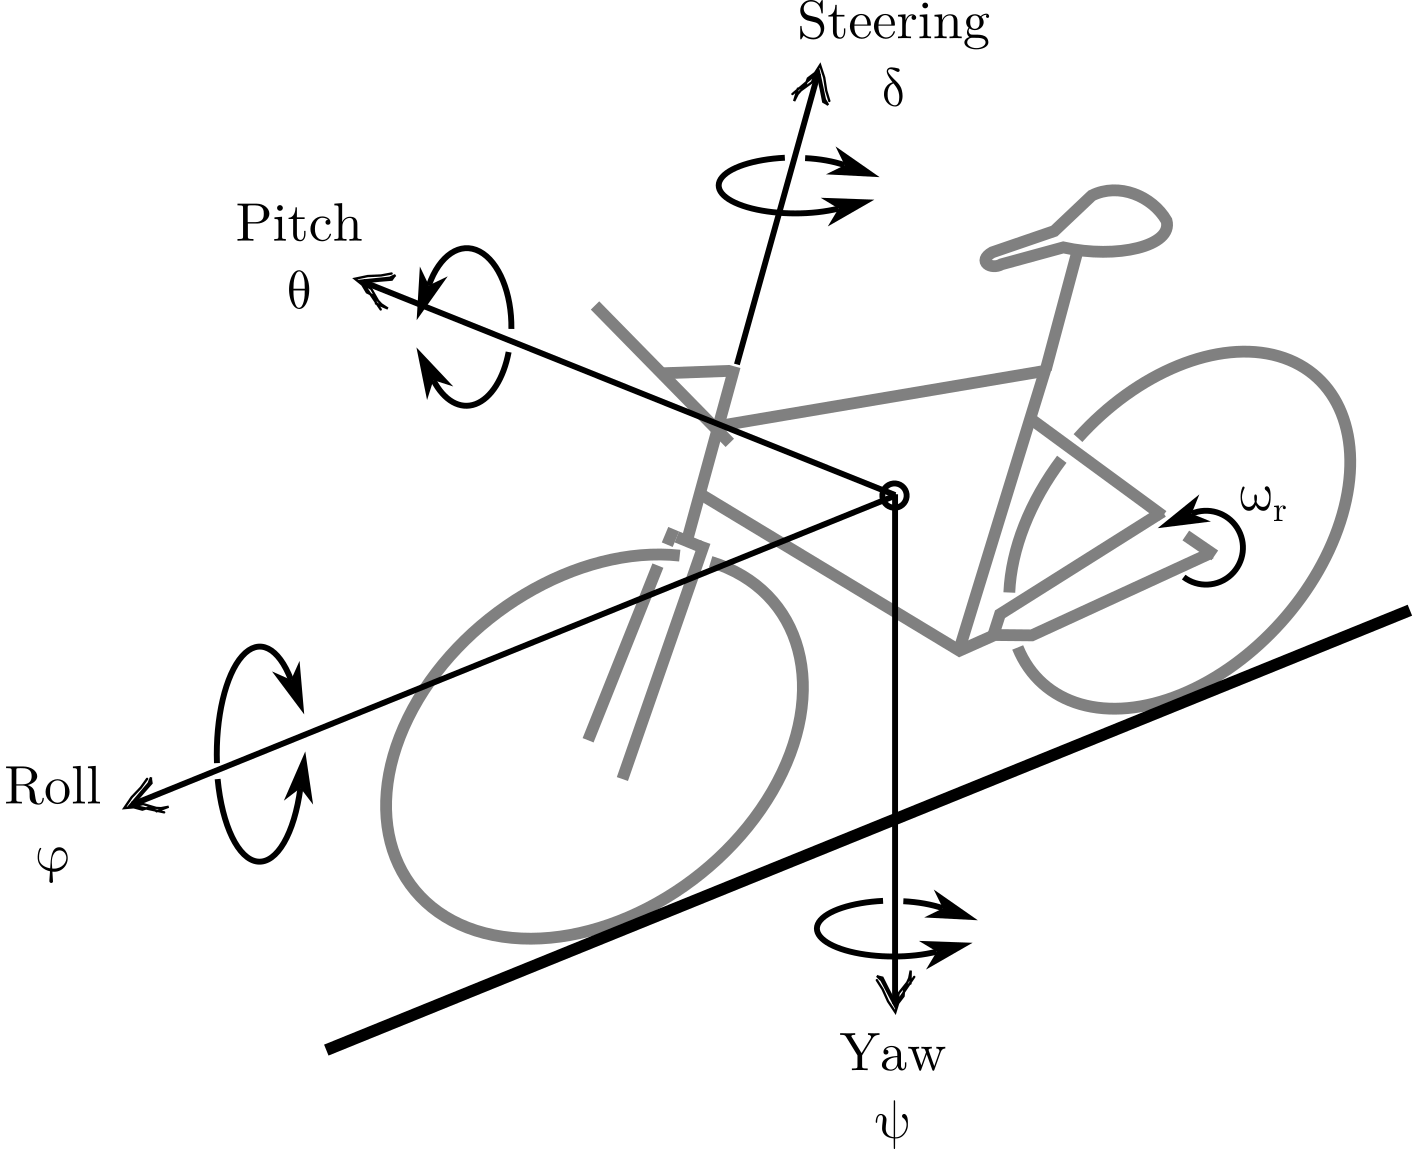
\includegraphics[width=0.5\linewidth]{Images/bike-dof-v0102.png}
    \caption{Rotational degrees of freedom of the bicycle}
    \label{fig: dof}
\end{figure}

Bicycles are human-powered two-wheeled vehicles that require lateral balance control to maintain an upright position, which dynamics have been a matter of scientific interest for more than 100 years \citep{Car99, Whi99}.
%
Thus, bicycle dynamics is the study of bicycle motion and stability governed by non-linear, coupled equations involving steering, tyre forces, and rider interaction.
%
The now-classical approach for its study considers the bicycle as a dynamical system composed of four rigid bodies: rear frame, front frame, and two wheels.
%
Assuming a rider rigidly attached to the bicycle, flat ground, non-slipping tyres and permanent contact with the ground, \cite{Mei07} presents the linearised equations of motion for the three-degree-of-freedom model.
%
These degrees of freedom are roll $\varphi$, steering $\delta$ and rear wheel rotation $\omega_r$ (see Figure \ref{fig: dof}).
%%


From the linear equations of motion, the stability of the bicycle is studied, showing a self-stable behaviour and three modes of vibration: weave, capsize, and caster.
%
Weave is a low-frequency oscillatory motion involving coupled roll and steer; capsize is a non-oscillatory motion similar to an inverted pendulum, and caster is the self-aligning motion of the front wheel.
%
From these three modes, weave and capsize are particularly interesting for their danger of loss of control when unstable.
%
Furthermore, if components compliance is included, wobble mode arises \citep{Sha71, Sch13}, which is an oscillatory motion of the steering, also dangerous when unstable \citep{Lim06}.
%%


Regarding the foundations of bicycles' self-stability, \cite{Koo11} demonstrated that it relies on mass distribution and steering coupled to lean angle.
%
Out of its self-stability speed range, bicycles rely on human control to maintain upright stable balance \citep{Koo13}.
%
To this end, the rider turns the steering into the falling side, which moves the contact point of the front wheel, shifting the equilibrium of the system.
%
Although most control actions come from the steering, at low speeds, the lower body starts to play a role in the control task \citep{Koo09}.
%
However, the steering is not the only control input, the rider makes use of the pedals and brakes to control longitudinal acceleration and deceleration, respectively.
%%


For the human, the task of riding a bicycle consists in first maintaining balance and then, following a desired trajectory.
%
In a crash scenario, it is understood that the failure occurs in the task of maintaining balance, due to the limits of control of the rider.
%
Hence, it is useful to understand how the human controls the bicycle in a given task.
%
For this goal, \cite{Hes12} considers a neuromuscular model for the rider's arms, with bandwidth limitations and gain selection that results in a controller with similar limits in control authority as a real rider.
%
In Hess' model, the rider receives feedback from the proprioceptive, vestibular and visual systems.
%
The proprioceptive loop refers to the information received from the body, such as the position of the limbs, and the vestibular system provides information about the orientation of the head and body in space.
%%


Being that steering is the main control input and the fastest loop, through proprioceptive feedback, on the model of \cite{Hes12}, its role is crucial for riding a bicycle.
%
Therefore, if the steering gets locked, the main balance control input disappears, losing the controllability of the system \citep{Koo11}.
%
Consequently, disturbances to the steering negatively affect the rider's ability to control the bicycle.
%%


In addition, bicycles are sensitive to aerodynamic forces, which are studied as a resultant force acting on the centre of pressure.
%
Aerodynamic forces acting opposite to bicycle motion are known as aerodynamic drag, and its study becomes interesting for enhancing cycling performance \citep{Deb11}.
%
Alternatively, forces acting on the lateral plane, such as cross winds, can affect the steering, generating large steering torque depending on front wheel aerodynamics \citep{Mao25}. 
%
For this reason, it is important to take them into account as a possible disturbance on the system in certain conditions.
%%


Concerning bicycles under longitudinal acceleration, their limitations rely on load transfer and tyre grip \citep{Lot21}.
%
On commuter riding conditions, the acceleration limit is far from being reached, different to the deceleration limit, which is subject to several factors.
%
For most bicycles, this limit is around $ 0.5 g$ \citep{Bec04, Fam20}, where $g$ is the gravitational acceleration.
%
Deceleration limit can be reached through brake actuation or collisions on the front wheel, where both cases result in pitch-over crashes \citep{Bre10}.
%
If tyre friction limit is reached, the rotational dynamics of the wheels change and the control of the vehicle becomes limited.
%
Therefore, acceleration of the system are a key indicator to assess the probability of a crash.
%%


Furthermore, tyre friction also plays a major role on cornering dynamics.
%
Single-track vehicles, such as bicycles and motorcycles, lean into the corner to maintain the equilibrium of forces, see Figure \ref{fig: cornering}.
%
These manoeuvres generate large lateral forces on the tyres, which are supported by friction between the rubber and the ground.
%
Hence, friction on the tyre-ground interface is a complex phenomenon of at least three mechanisms: adhesion, deformation and wear \citep{Han03}.
%
Adhesion refers to the bonding between both surfaces, while deformation is the capability of the tyre to adapt to the road irregularities.
%
Along, wear occurs when local stress on the tyre surpasses its elastic limit, causing tearing and dissipating energy, which results in friction.
%
Therefore, when there is an external agent on this interface, such as water, dust or another layer of material, tyre friction relies only on deformation \citep{Mic01}.
%%


Tyre friction is a non-linear behaviour on lateral and longitudinal loads, which has a saturation limit at a given force.
%
Within the operating range of a tyre, the angle between the direction of the motion of the wheel and the ground is known as `slip angle'.
%
Depending on the slip angle of the front and rear axle, the vehicle can present an understeering, neutral, or oversteering behaviour \citep{Cos06}.
%
Understeering occurs when front side-slip is larger than rear, therefore, the vehicle turns less than expected.
%
Contrarily, oversteering occurs when rear side-slip is larger than the front, thus, the vehicle turns more than the steering input.
%
When both slips are balanced, the vehicle behaves neutral, following the path determined by the user through the steering.
%
Thus, the cornering behaviour of the bicycle will influence the crash configuration when the tyre-ground interface mechanism fails.
%%


Consequently, when the saturation limit is reached, the tyre starts to exhibit a phenomenon called `skidding'. 
%
The extent of loss of grip will lead to different crash configurations, as explained in Section \ref{subsec: crash motion}, which is particularly interesting to understand single-cyclist crashes.
%
Therefore, cornering and tyre dynamics are fundamental to understand bicycle crashes.
%%

\begin{figure}
    \centering
    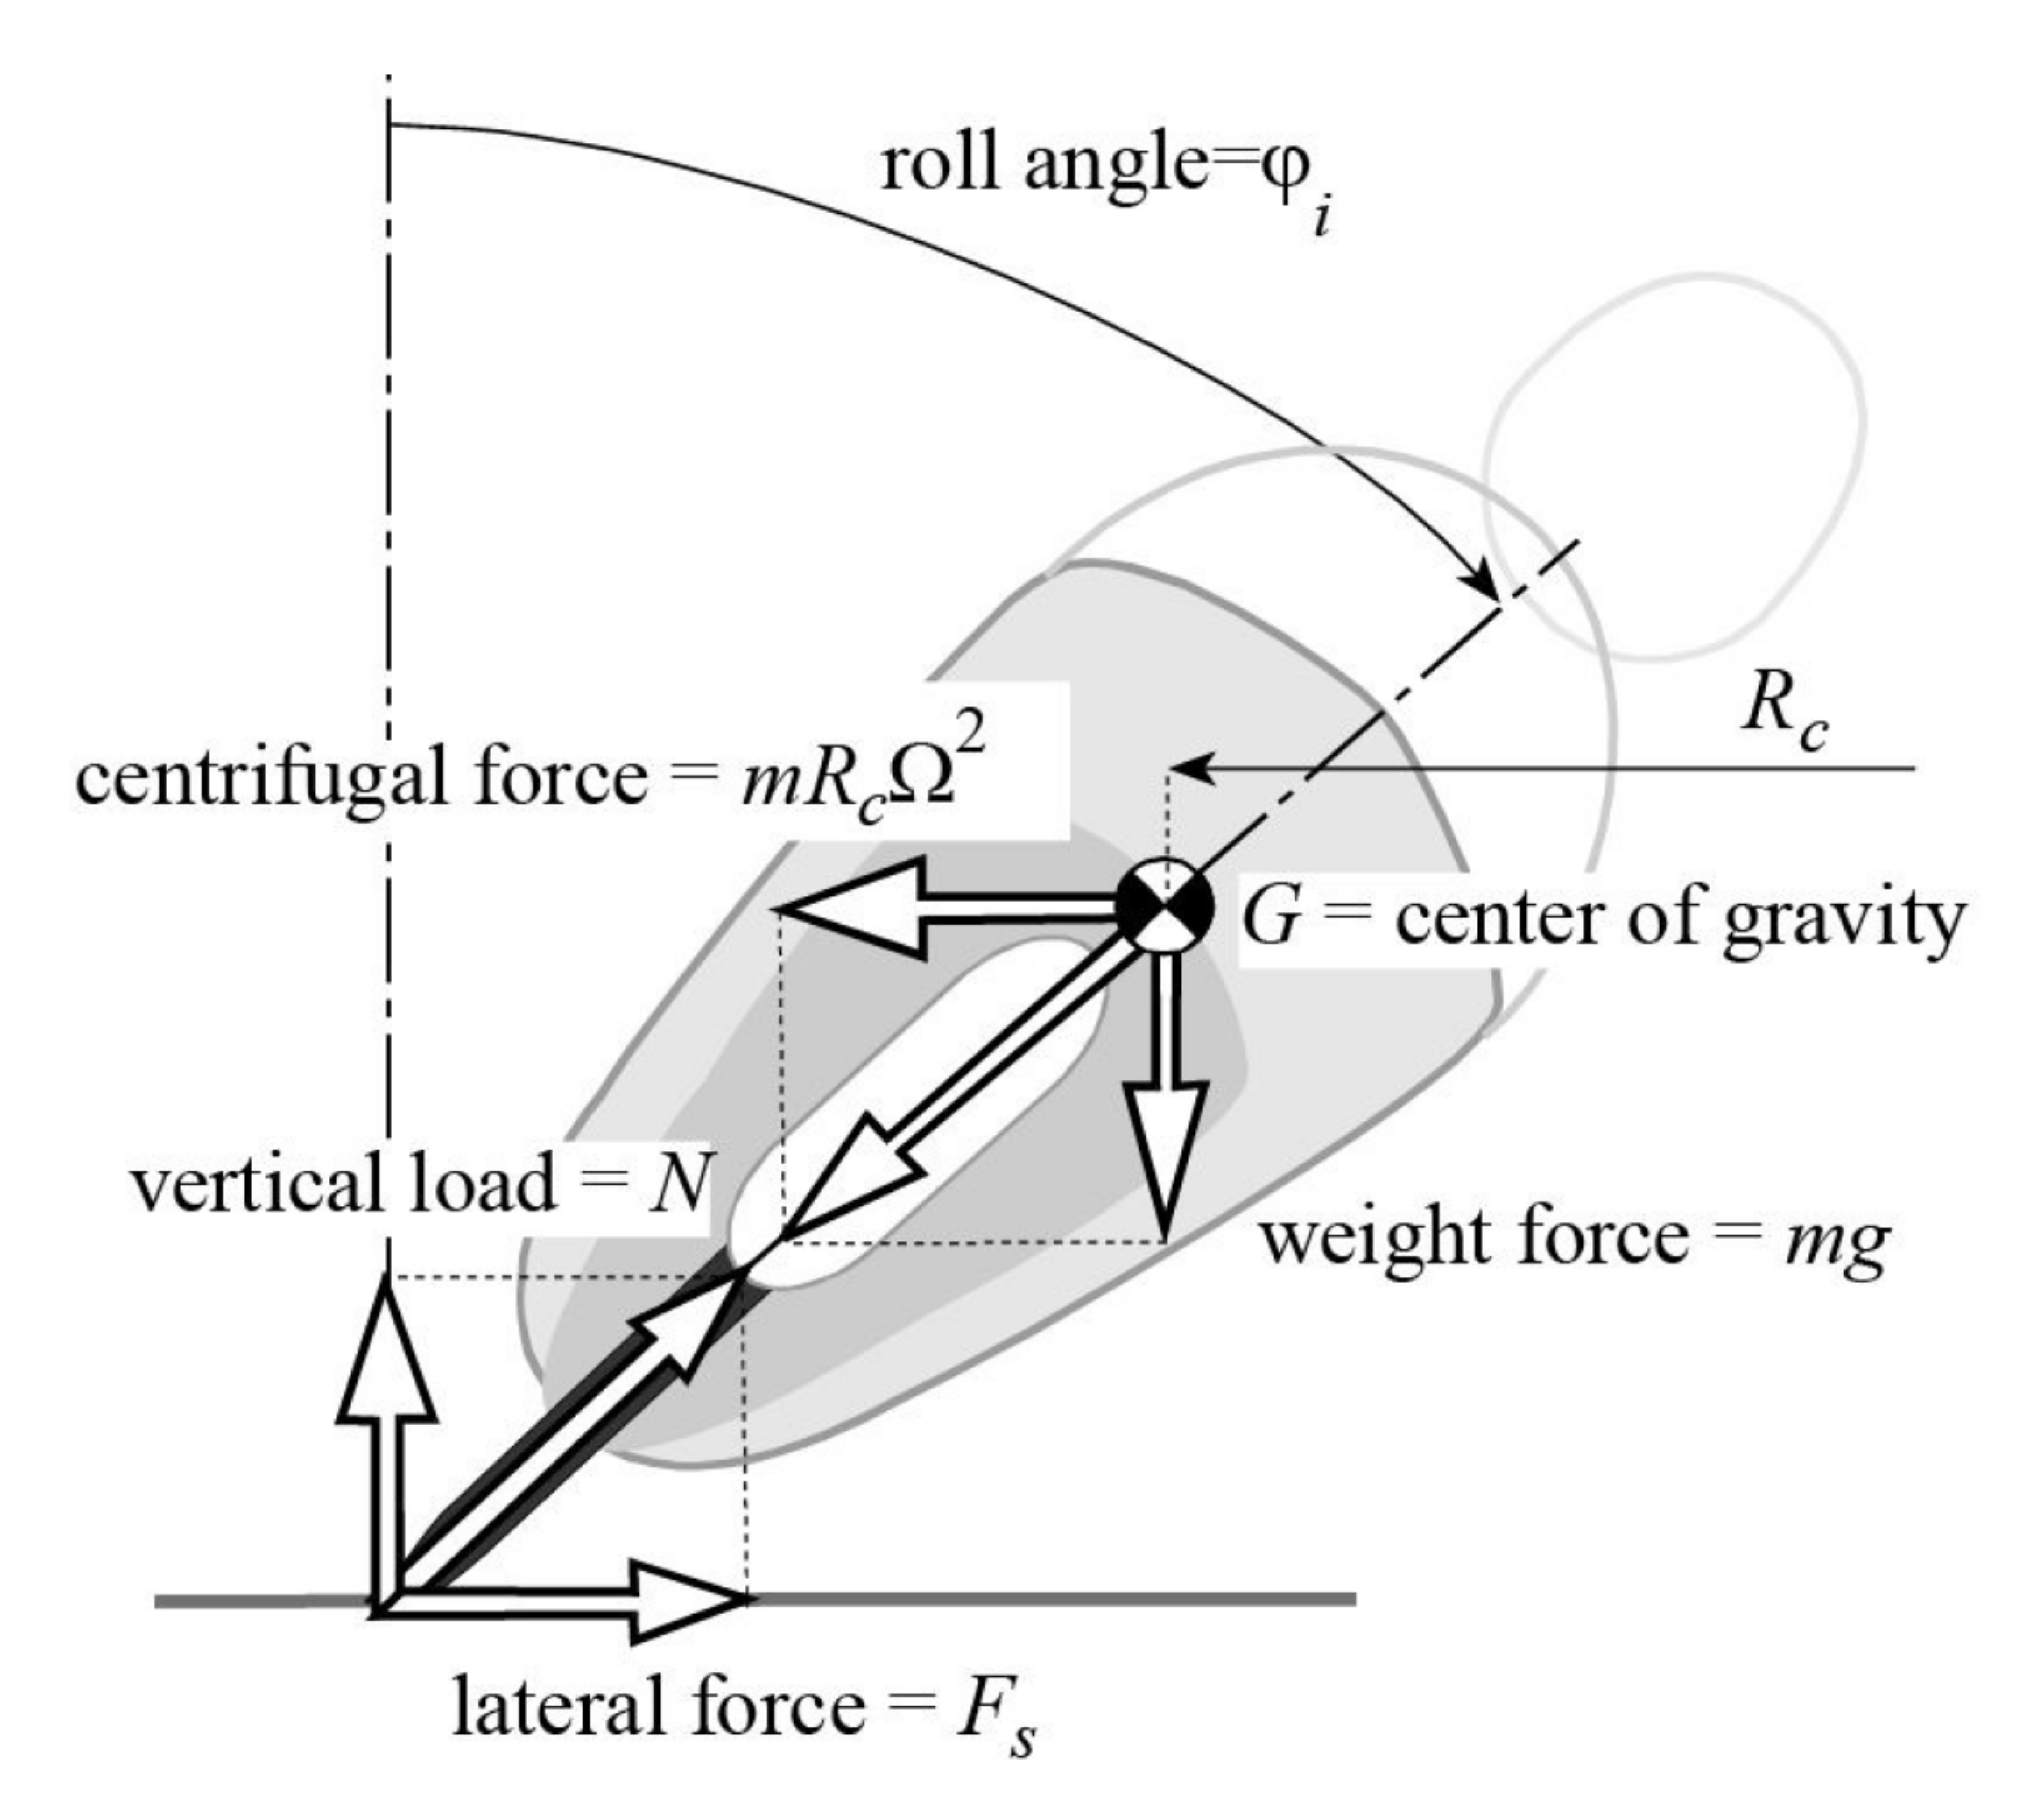
\includegraphics[width=0.5\linewidth]{Images/cossalter_cornering.png}
    \caption{Steady turning: roll angle of the motorcycle equipped with zero thickness tires. From \cite{Cos06}.}
    \label{fig: cornering}
\end{figure}


In summary, bicycles can be self-stable but require human control to maintain balance over a wider range of speeds.
%
This human control is studied as dependent on the feedback from the two main degrees of freedom of the system.
%
Within the motion of the system, we find longitudinal and lateral dynamics that face different challenges in their interaction with the environment.
%
Thus, the bicycle-rider system is a complex dynamical system that requires a deep understanding of its dynamics to assess its failure mechanisms.
%%


\subsection{Single-cyclist crash anatomy} \label{subsec: crash anatomy}
%
A single-cyclist crash is the result of the rider losing control of the bicycle, which is the inability of the user to manoeuvre the vehicle to a desired state.
%
\cite{Ful05} describes, in his task-capability interface model, the loss of control as a relation between task demand and rider capability.
%
When the task demand surpasses rider's capability, the rider loses control and the crash occurs.
%
This model considers physical characteristics and knowledge of the driver on what to do under determined circumstances to define the boundaries of its capability.
%
However, this capacity is also affected by other factors related to the circumstance, such as awareness, emotion, and fatigue, among others.
%
On the other hand, task-demanding elements encompass travelling speed, environmental factors, such as road characteristics and other road users.
%
Of these factors, the driver has direct control of the travelling speed, achieving a balance between driver capacity and their awareness of the task.
%
However, a major difference between car drivers and bicycle riders is that the latter has an extra task: maintaining lateral balance.
%
While car drivers can reduce task demand by decreasing speed, for bicycle riders, decreasing the speed can increase stabilisation requirements, and therefore, task demand increases \citep{Koo11, Sch13, Vla15}.
%
In general, the theory shows an almost constant gap between driver capability and changing task demands, which should not surpass the critical threshold.
%%


Now, when task demands surpass the rider's capability, a critical scenario is triggered.
%
This scenario becomes a loss of control and a possible crash, depending on the extent of the loss of control \citep{Gil23}.
%
Factors that increase task demand in critical scenarios are known in the literature; the most repeated are skidding, low-speed riding, braking, `loss of control', and collision with an object.
%
These events require a precise and quick response from the rider, which can be assumed as a high-demand task in Fullner's model.
%
It is important to note that in a high-demand task, the user can still have control over the vehicle.
%
However, the user is unable to complete the task, which is, for example, avoiding an obstacle.
%%


\subsubsection{Crash dynamics} \label{subsec: crash dynamics}
%
Crash dynamics is the study of the forces, energy transfer, and motion during the loss of control in the rider-bicycle system.
%
It encompasses the analysis of how the vehicle and its occupant respond to impacts, considering factors like speed, mass, and direction.
%
Thus, a crash is defined as a sudden and unintended event that disrupts the normal and controlled motion of the rider-vehicle system \citep{Wie18}.
%
The analysis of crash dynamics is typically divided into three distinct phases: pre-crash, crash, and post-crash motion \citep{Par01}.
%%


The pre-crash phase begins with a perturbation and ends when the system loses its rideability.
%
During this phase, the system's kinetic and potential energy, along with rider control, determine the trajectory of the bicycle.
%
In this stage, energy is rapidly and uncontrolledly redistributed, modifying the behaviour of the system.
%%


Then, the crash phase is composed of the uncontrolled motions as a result of the failure mechanisms, together with protective responses from the rider.
%
As previously shown, bicycle's motion in a three-dimensional space are fundamental to explain crash motions.
%
The literature about bicycles discusses three types of characteristic crash motions: pitch-over \citep{Bre10}, roll-over \citep{Sch21} and skid-out \citep{Gil21a}.
%
However, the literature on motorcycle crashes adds low-side and high-side motions \citep{Cos06, Cos07, Pet20, Ros17}.
%
These concepts are further explained and discussed in Section \ref{sec: crash motion}.
%%



The post-crash phase is typically brief in single-cyclist crashes, due to the inherent instability of the bicycle, it will tend to rest immediately after the crash itelf.
%
This phase is defined by the moment the bicycle contacts the ground with components other than the wheels \citep{Llo16}.
%%


\subsection{Single-cyclist crash classifications} \label{subsec: classifications}
%
Currently, studies on single-cyclist crashes are based on the available data, which is mainly descriptive from hospital, police, and insurance reports.
%
Within these studies, \cite{Sch12} presents a classification by reviewing the existent description of single-cyclist crashes, along with the basic concepts to understand bicycle dynamics.
%
Then, he divides the three components needed for a crash: rider, bicycle, environment, and includes the category `other', analogous to the analysis for car crashes made by \cite{Fel76}.
%
They revises the known crash circumstances and factors, such as age, amount of bicycle usage, road surface, type of bicycle, speed, among others.
%
The data collected came from surveys sent to people who attended to the hospital due to a bicycle crash within the two prior months.
%
The results of the classification based on survey responses showed 85\% of agreement between two researchers.
%
It concludes that single-cyclist crashes can be categorized according to direct causes, and for future work, recommends to research specific crash types.
%%


Then, we find a four-layer approach from \cite{Gil21a}, using direct causes and fall types, which allows to analyse the kinematic form of cyclist's falls.
%
Direct causes are based on \cite{Sch12} and \cite{Utr20}, which create the crash scenario depending if it is composed on one or two direct causes.
%
Then, Gildea takes into account the common factors found on the literature, such as the mentioned in Table~\ref{tab: known mechanisms}.
%
At last, he distinguishes between three fall types: pitch-over, topple-over, and skid-out.
%
Where pitch-over refers to a sudden deceleration causing the cyclist to be projected forwards due to inertia.
%
Topple-over is the cyclist falling to the side, and skid-out is when the tyre loses traction and the bicycle falls beneath the rider. 
%
Using this methodology, it is possible to cluster the events and compare them with the outcomes of the crash.
%%


\cite{Sch21} aimed to develop a crash detection system, which uses measured accelerations on the bicycle to detect the events.
%
To identify events where a crash occurs, he develops a hierarchy based on his definition of stages in a crash, defining four classes: riding state, collision, ground hit and tipping over.
%
All of them have sub-states, which combined result in 60 possible events, where 38 are categorised as crashes.
%
Interestingly, the last layer of this method distinguishes between nose over (pitch-over), tip over (roll-over), and upright bicycle.
%
Nevertheless, this classification does not provide a detailed description of the crashes, which constitutes part of the future work they discussed.
%%


\cite{Gil23a} develops a video-based crash detection system.
%
For this reason, he uses the proposed categorisation of \cite{Gil21a} and identifies the extent of the loss of control.
%
With this, a new level of category is created: minor, substantial and complete loss of control.
%
In minor loss of control, the rider is able to recover the balance and continue riding.
%
Substantial loss of control refers to the situation where the rider loses control and needs to stop or dismount before continuing its ride.
%
Finally, complete loss of control refers to the events where the rider falls to the ground.
%%



Although Gildea's work analyses crash motions focused on the human, there is still a lack of information about the dynamics of the bicycle prior and leading to the crash.
%
Across the studies, the conclusion is that the most frequent causes of single-cyclist crashes are skidding, loss of control by braking or steering manoeuvres, and external perturbations such as hitting a kerb \citep{Sch12, Her18, Utr20, Alg22}.
%
Moreover, the way of interaction with the environment can increase the risk, e.g. the angle of crossing a tram line \citep{Gil23}.
%
However, there is no information about which one of the wheels slips, longitudinal or lateral velocity, steering angle, braking force, etc.
%%
% Therefore, it is necessary to provide a classification that highlights this gap and invites to further research.



\subsubsection{Known mechanisms}
%
\begin{landscape}
\sloppy 

\begin{longtable}{@{}%
  >{\raggedright\bfseries\arraybackslash}p{60mm}%
  >{\justifying\arraybackslash}p{140mm}%
  @{\hspace{6mm}}% extra gap between middle and right columns
  >{\footnotesize\raggedright\arraybackslash}p{51mm}@{}}


\toprule
\textbf{Type} & \textbf{Description} & \textbf{Discussed in} \\
\midrule
\endfirsthead

\toprule
\textbf{Type} & \textbf{Description} & \textbf{Discussed in} \\
\midrule
\endhead

\midrule
\multicolumn{3}{r}{\footnotesize Continued on next page} \\
\caption{Known crash mechanisms and their definition on the literature.}
\label{tab: known mechanisms}
\endfoot

\bottomrule
\endlastfoot

Braking mistakes & brake over-actuation can produce wheel lock, which can end in a pitch-over crash or losing grip in one or both of the tyres & \cite{Alg22, Gil21, Her18, Ohl19, Sch12} \\
Caught in track & refers to one of the wheels falling on the gap of tram tracks, which locks the steering if the front wheel is locked & \cite{Alg22} \\
Collision & collision with objects on the road, these can be objects temporarily or permanently placed there & \cite{Bec19, De14, Gil21, Her18} \\
Crossing a threshold & the wheel hits a threshold and produces a mechanisms similar to tram track interaction or pothole striking & \cite{Her18} \\
Evasive manoeuvre & the rider executes a manoeuvre to avoid an obstacle and loses control & \cite{Alg22, De14, Gil21, Her18, Ohl19, Sch12, Utr20} \\
Fall & no further definition on the literature & \cite{Utr20} \\
Front wheel hit & the front wheel hits the curb or an object collides with it in on the lateral plane & \cite{Gil21, Sch12, Utr20} \\
Getting on/off the bicycle & users starting the ride or stopping, this involves the manoeuvre from standing to sit on the bicycle at low speeds, which increases balance task demand and the rider places its weight mainly on the pedals & \cite{Alg22, Boe17, Ohl19, Utr20} \\
Kerb hit & when the bicycle reaches the edge of the road, the wheels collide with the kerb, exerting an unexpected force on the system & \cite{Boe17, Gil21, Sch12, Utr20} \\
Loss of control on a descent & no further definition on the literature & \cite{Bec19} \\
Low speed loss of balance & at low speeds, bicycles have higher balance requirements from the user, thus, if the rider is not capable of controlling the steering properly, it produces a crash & \cite{Ohl19, Sch12} \\
Mechanical malfunction & any mechanical failure from the bicycle, non working brakes, broken chain, among others & \cite{Alg22, Bec19, Gil21, Ohl19, Sch12} \\
Object on the road & discussed as a type of collision & \cite{Alg22, Bec19, Boe17, Gil21, Her18, Sch12} \\
Other perturbations & external forces that can not be attributed to infrastructure or induced rider perturbations & \cite{Sch12} \\
Riding off the road & the rider is unable to maintain the desired trajectory on the road, which results with the bicycle reaching the edge and colliding with the kerb or falling on the non-road area & \cite{Gil21, Her18, Sch12, Utr20} \\
Road surface conditions & uneven roads or slippery surfaces such as wet leaves, gravel, ice, or water on the road & \cite{Gil21, Her18} \\
Skidding & one or both tyres suddenly lose grip & \cite{Alg22, Bec19, Her18, Ohl19, Sch12, Utr20} \\
Slipping off pedals & when the rider is exerting a high-power input into the system, if the foot-pedal joint fails, the rider suddenly changes its load distribution and the contact points with the bicycle & \cite{Her18, Utr20} \\
Something caught on the wheel & objects getting into one of the wheels suddenly locking it & \cite{Alg22, Ohl19} \\
Striking pothole & when the wheel strikes a pothole, the contact point changes, diminishing the available grip, or causing an excessive deceleration & \cite{Bec19} \\
Stunt & refers to doing stunts where the standard riding configuration changes, such as one of the wheels lifts from the ground, or riding without one or both hands & \cite{Gil21, Sch12} \\
Tram track interaction & the two mechanisms discussed for tram track interaction are one of the wheels getting locked, or losing grip due to the lower available friction of track surfaces & \cite{Bec19, Her18, Ohl19} \\
Turning mistake & no further description on the literature & \cite{Gil21} \\
Unable to keep balance & the rider is not capable of maintaining the bicycle in upright position & \cite{Her18} \\
Uneven road & uneven road surfaces such as cobblestones or improperly maintained roads, cause the wheels to loose contact with the ground & \cite{Alg22, Gil21, Sch12} \\
\end{longtable}
\end{landscape}

\normalsize


\subsection{Bicycle dynamics-based crash classification} \label{subsec: newclassification}
%
\begin{figure}
    \begin{subfigure}[t]{.45\textwidth}
        \centering
        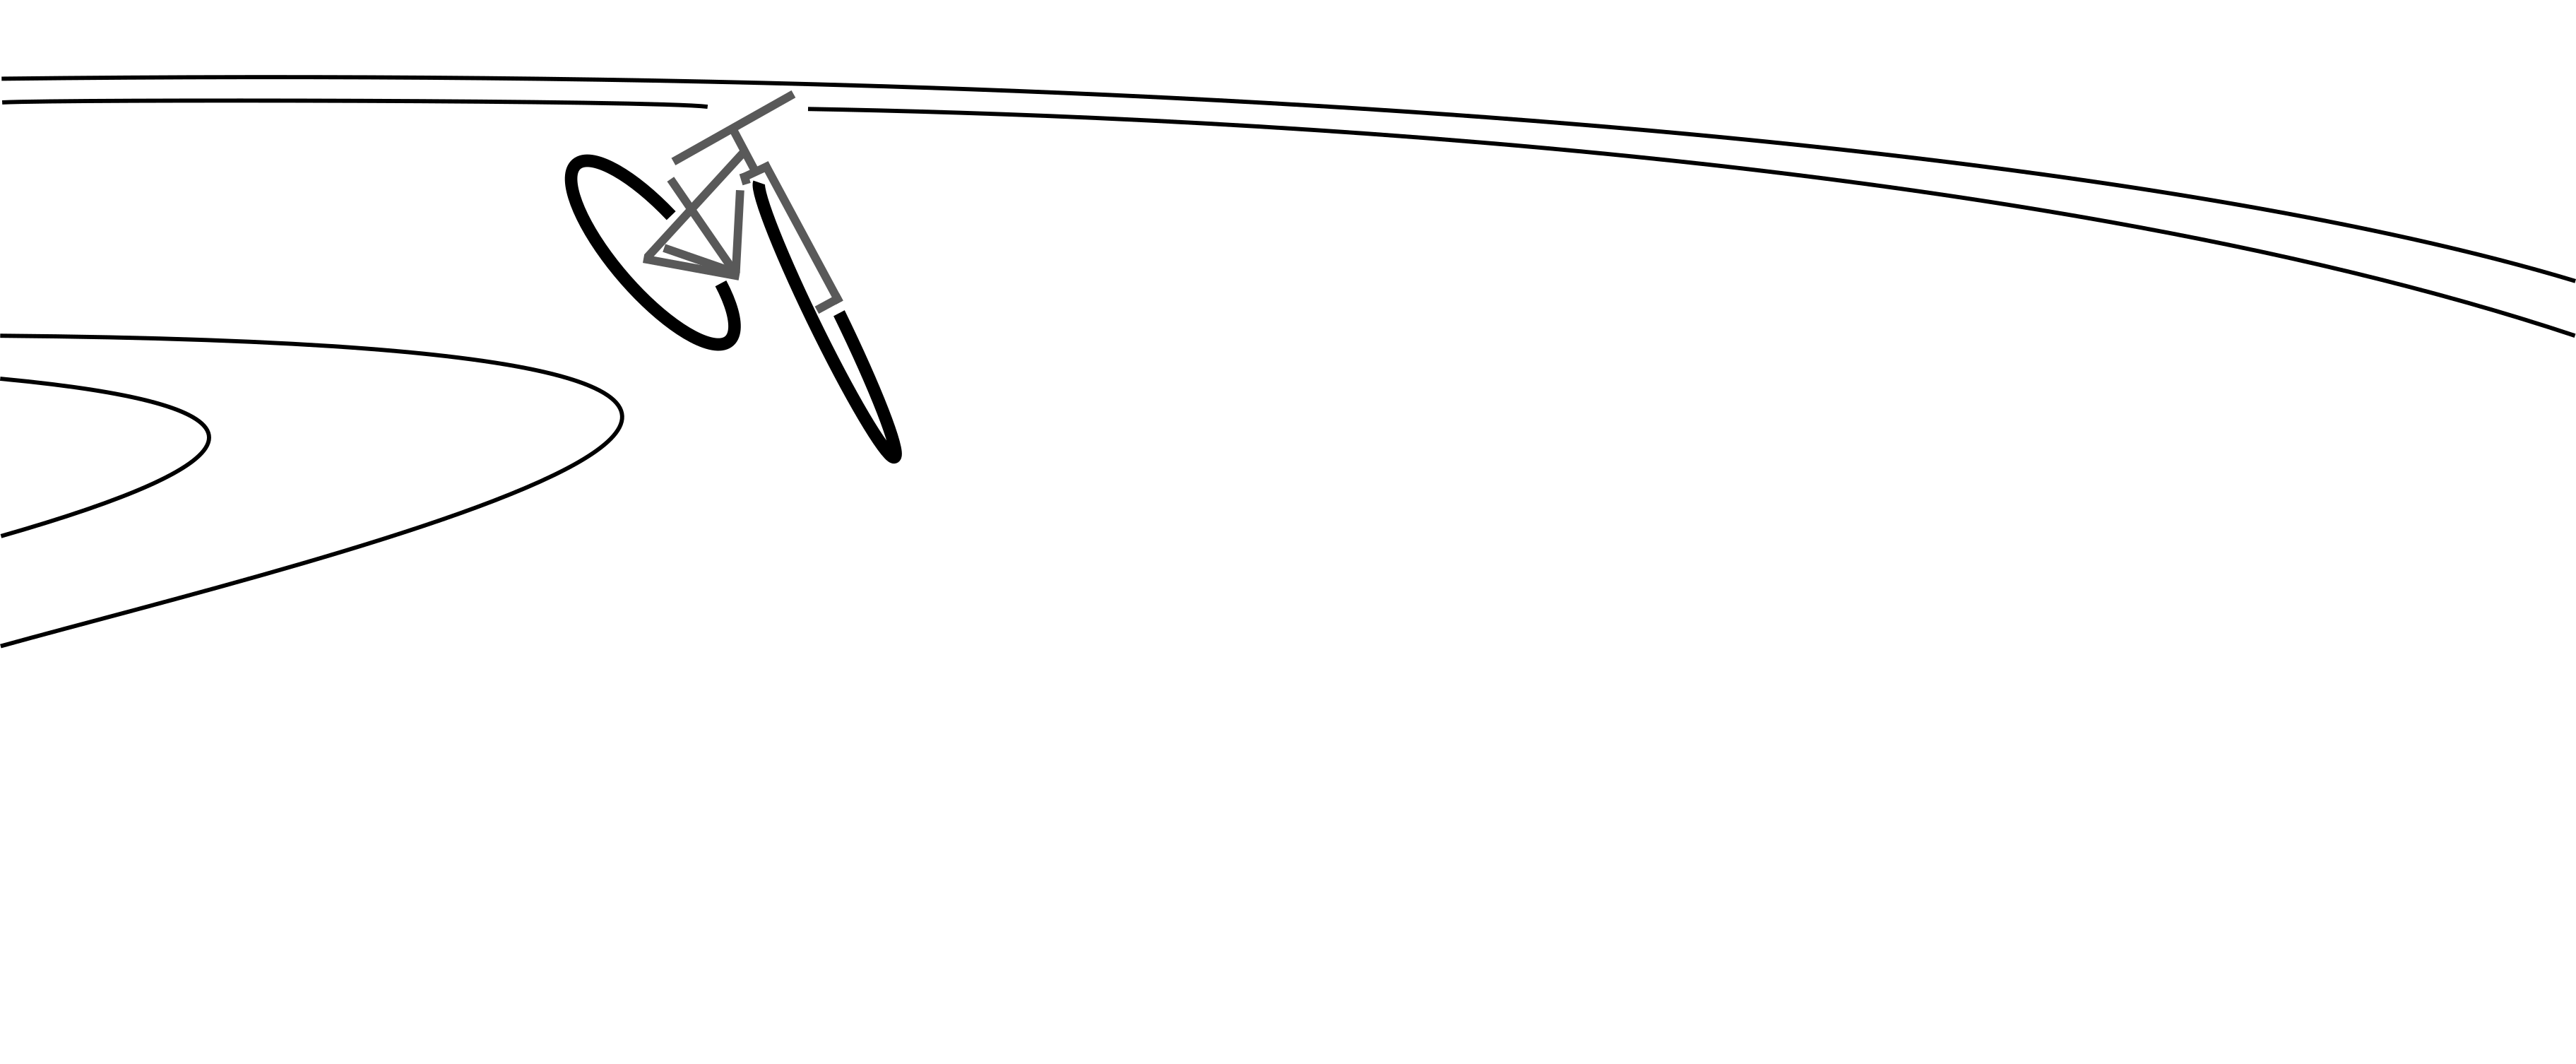
\includegraphics[width=\linewidth]{Images/turn.png}
        \caption{First stage: vehicle turning to the right with both wheels following the desired path.}
    \end{subfigure}
    \hfill
    \begin{subfigure}[t]{.45\textwidth}
        \centering
        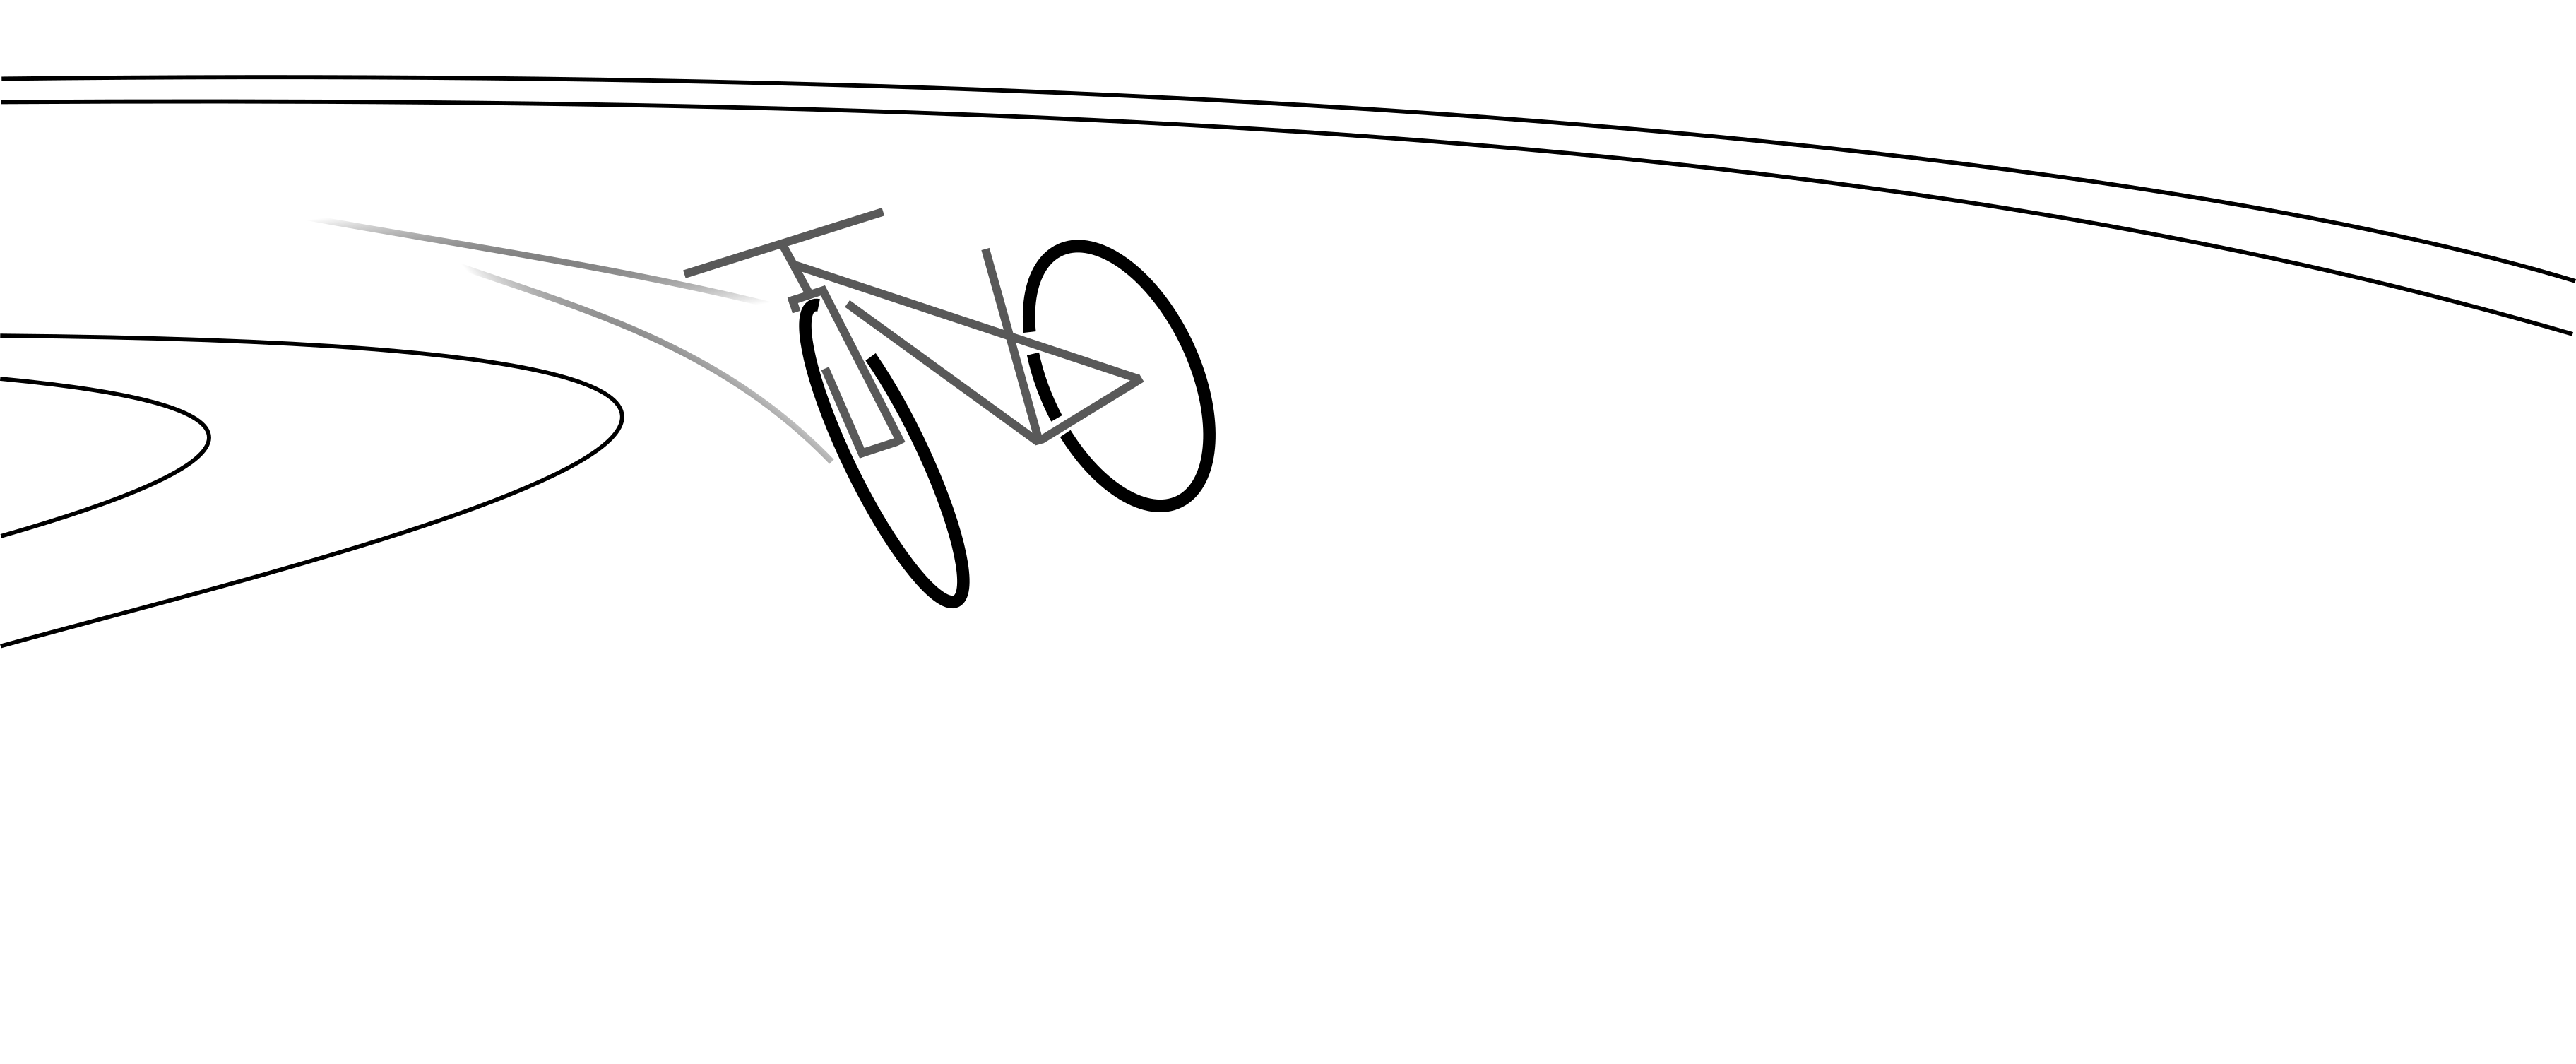
\includegraphics[width=\linewidth]{Images/hs-skid.png}
        \caption{Second stage: the rear wheel loses grip and the vehicle turns more than rider input. External excitation with tyre friction as failure mechanism, which may be caused by any grip-degenerating agent on the road surface.}
    \end{subfigure}

    \medskip

    \begin{subfigure}[t]{.45\textwidth}
        \centering
        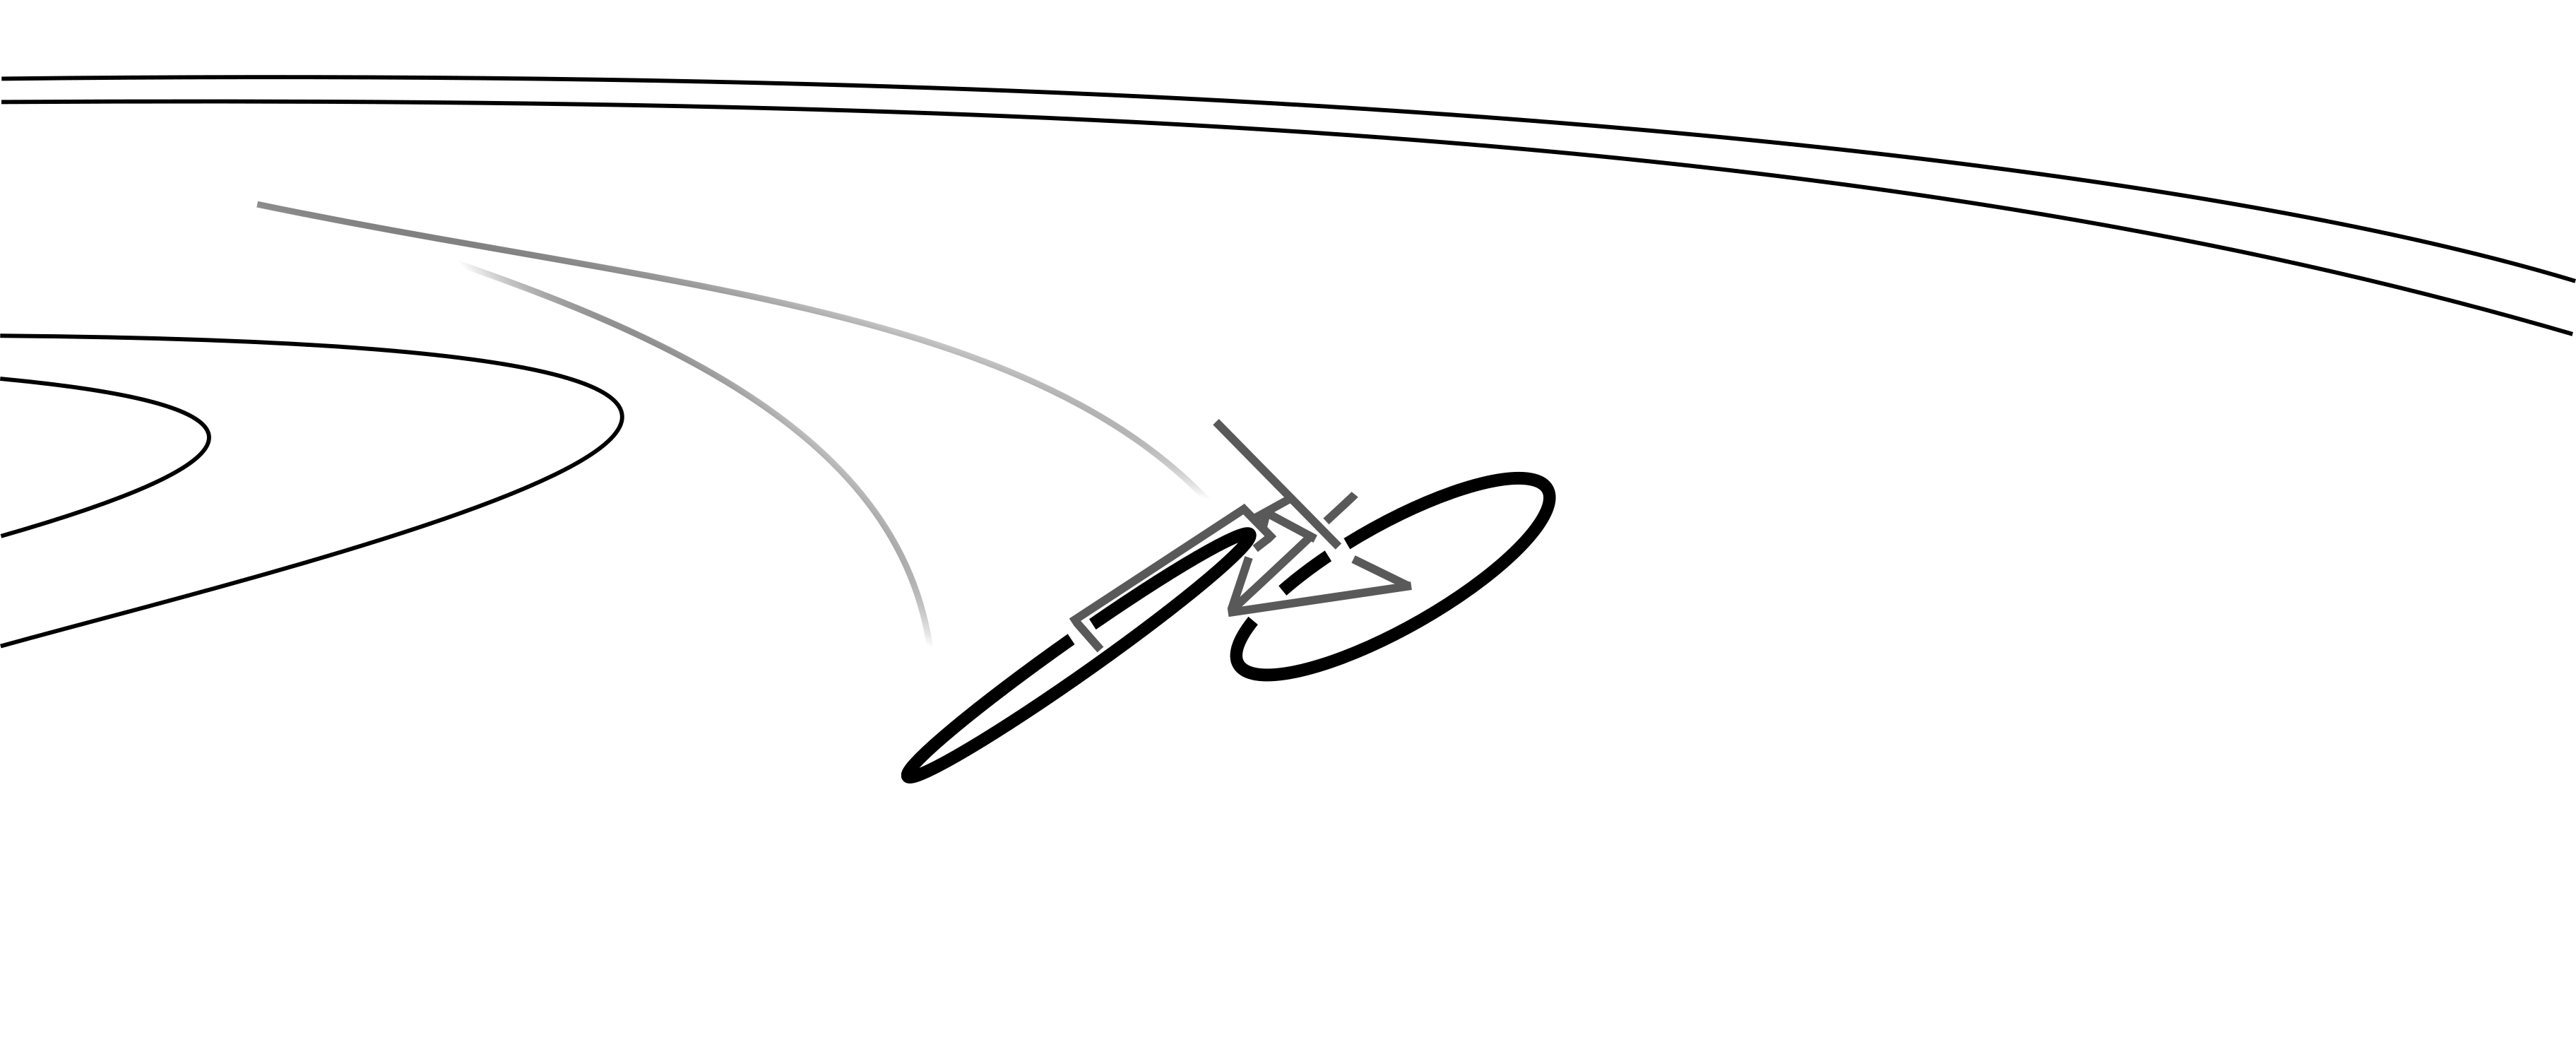
\includegraphics[width=\linewidth]{Images/hs-lock.png}
        \caption{Third stage: the rear wheel suddenly recovers grip, creating large rotational acceleration that ejects the rider.}
    \end{subfigure}
    \hfill
    \begin{subfigure}[t]{.45\textwidth}
        \centering
        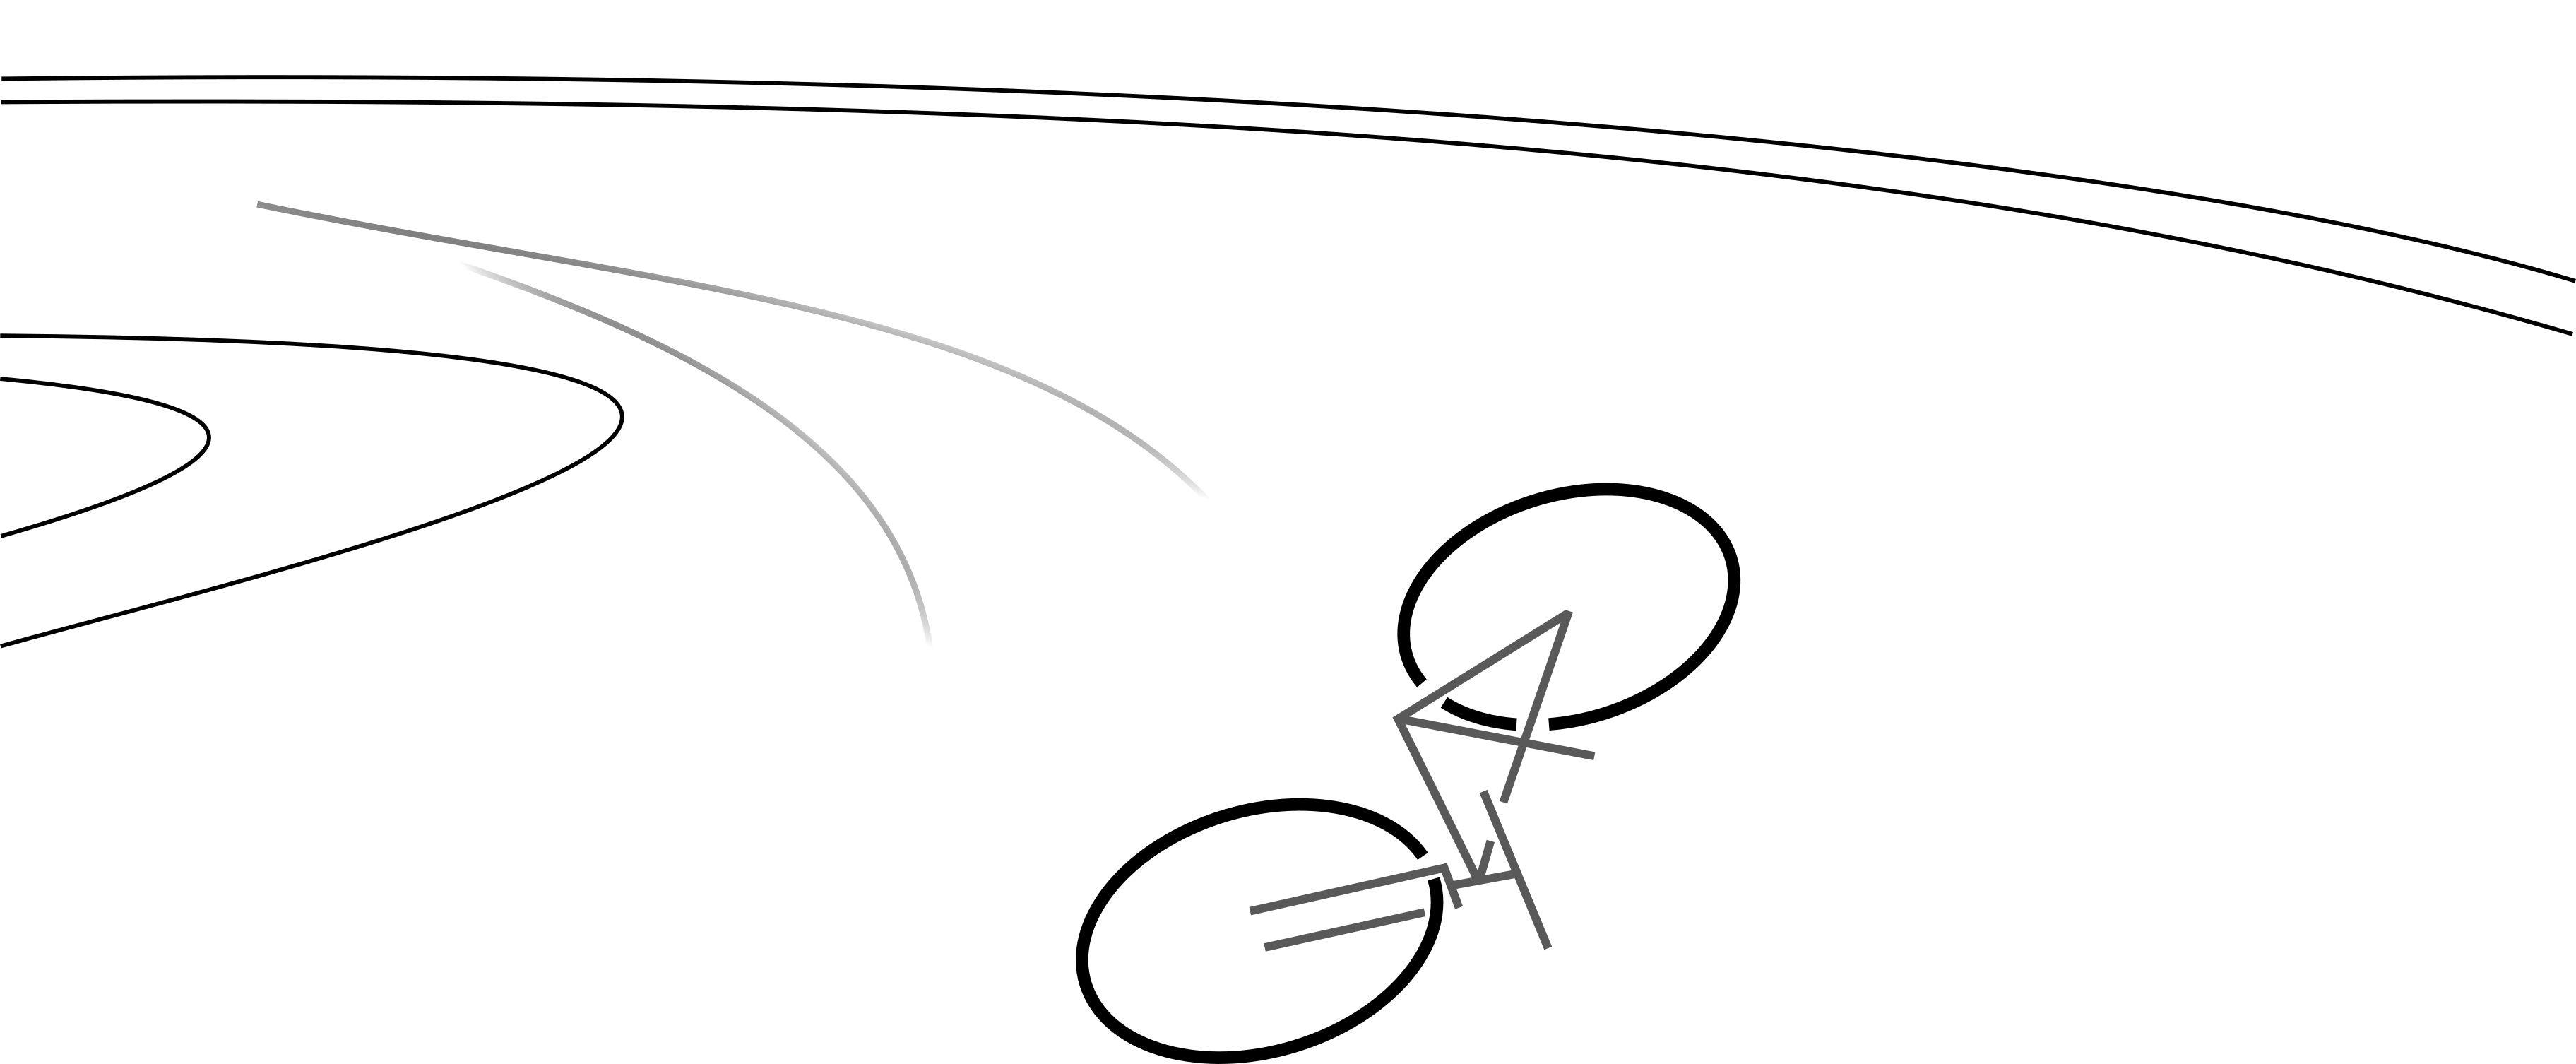
\includegraphics[width=\linewidth]{Images/hs-fall.png}
        \caption{Fourth stage: the rider is disconnected from the vehicle and the control is completely lost.}
    \end{subfigure}
    \caption{High-side crash schematic sequence.}
    \label{fig: highside}
\end{figure}

\begin{figure}
    \centering
    \begin{subfigure}[t]{.45\textwidth}
        \centering
        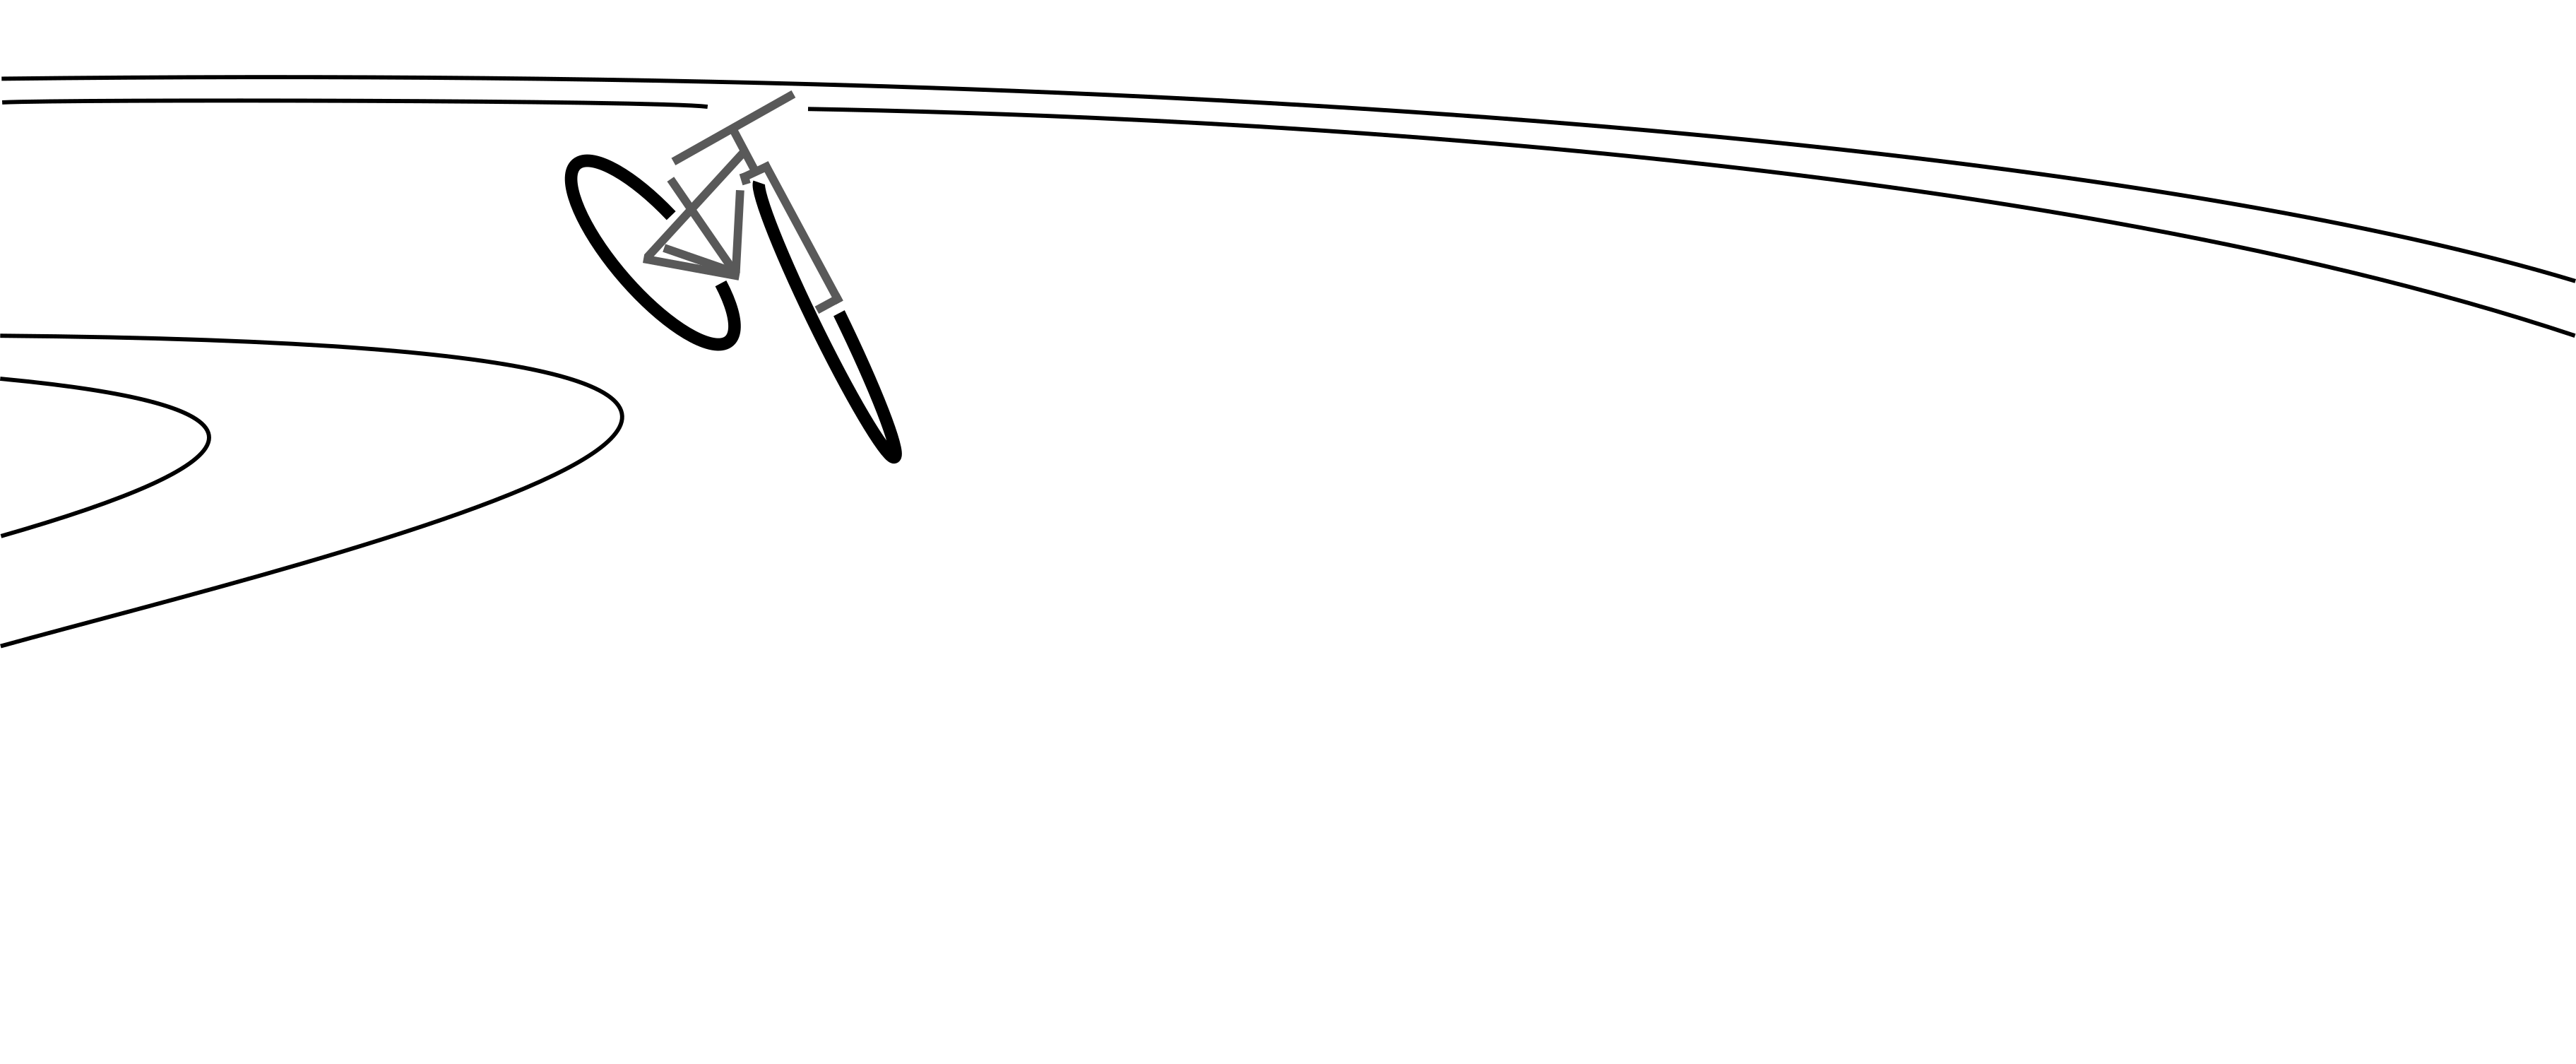
\includegraphics[width=\linewidth]{Images/turn.png}
        \caption{First stage: vehicle turning to the right with both wheels following the desired path.}
    \end{subfigure}
    \hfill
    \begin{subfigure}[t]{.45\textwidth}
        \centering
        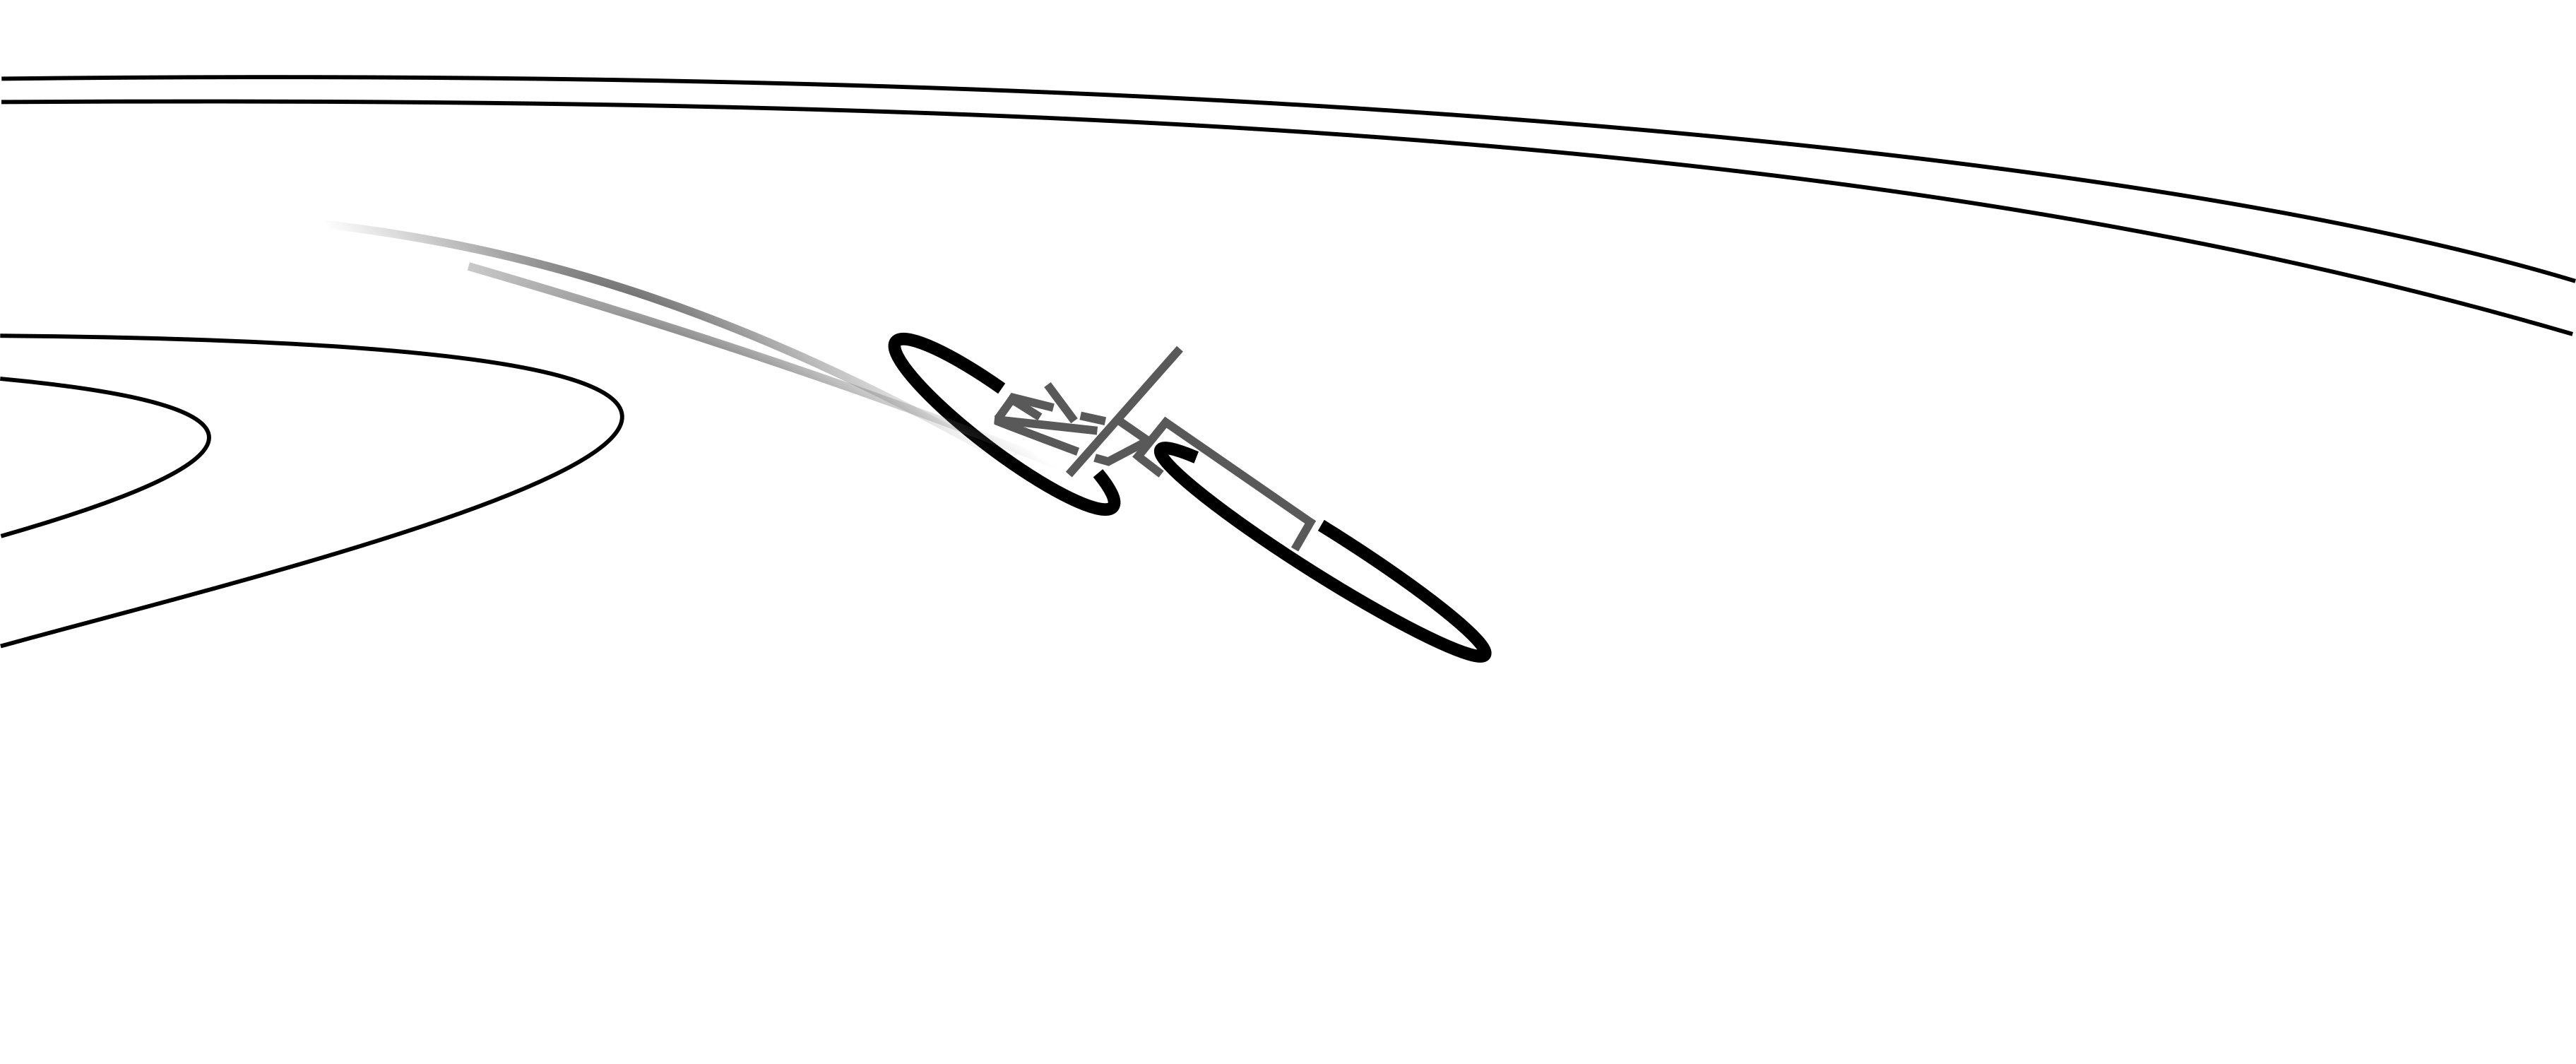
\includegraphics[width=\linewidth]{Images/ls-skid.png}
        \caption{Second stage: the front wheel loses grip, wheel dynamics change and modify the trajectory, turning less than the rider input.}
    \end{subfigure}
    \vspace{1em}
    \begin{subfigure}[t]{.45\textwidth}
        \centering
        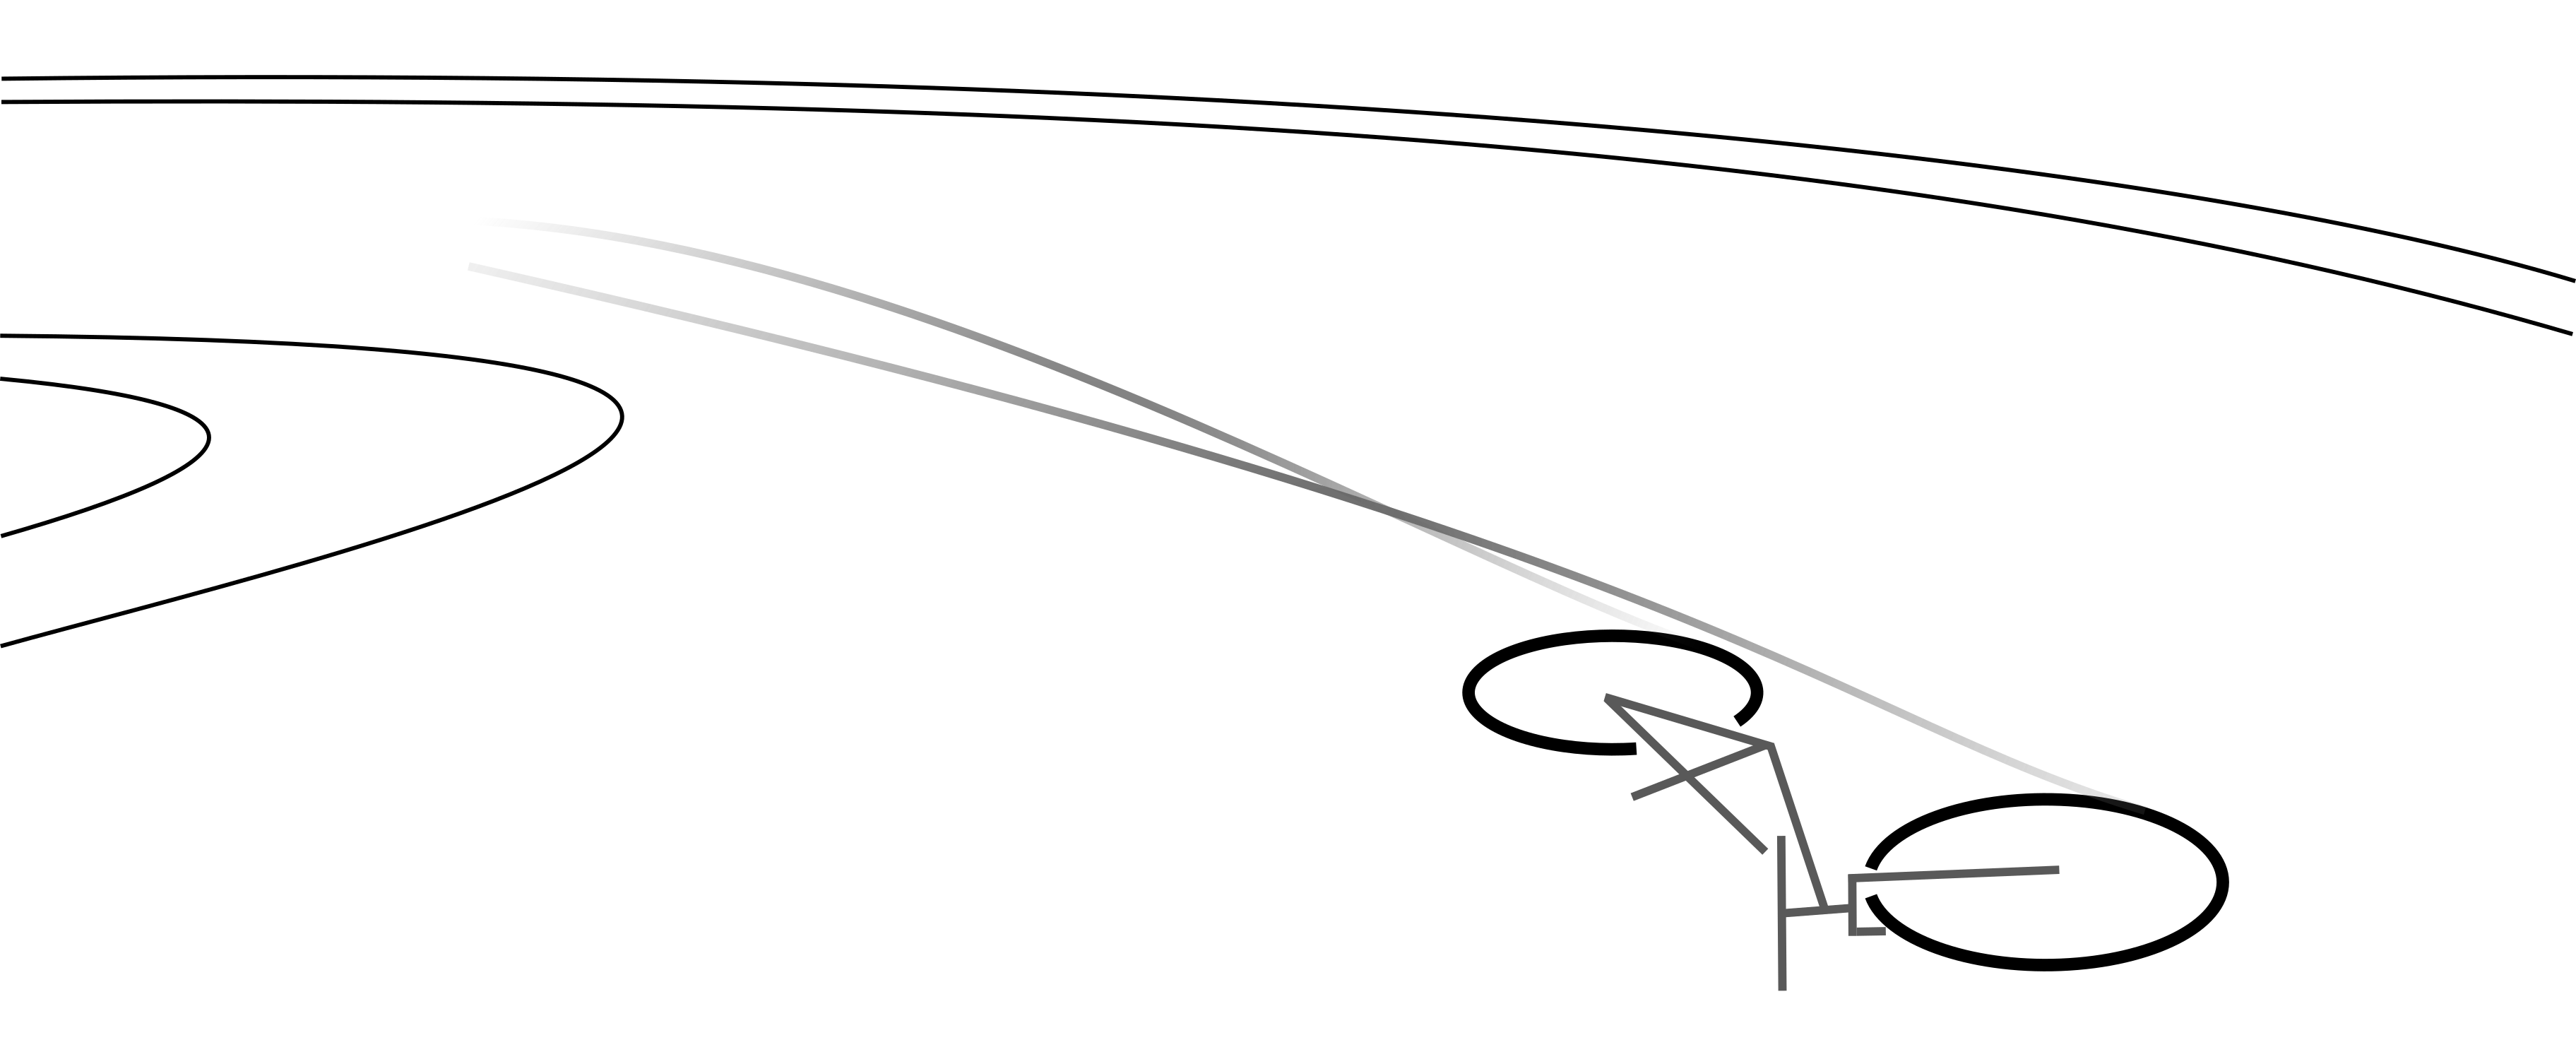
\includegraphics[width=\linewidth]{Images/ls-fall.png}
        \caption{Third stage: cornering dynamics fail and the bicycle follows an uncontrollable roll rate.}
    \end{subfigure}
    \caption{low-side crash schematic sequence.}
    \label{fig: lowside}
\end{figure}

\begin{figure}[h]
    \centering
    \begin{subfigure}[t]{0.32\textwidth}
        \centering
        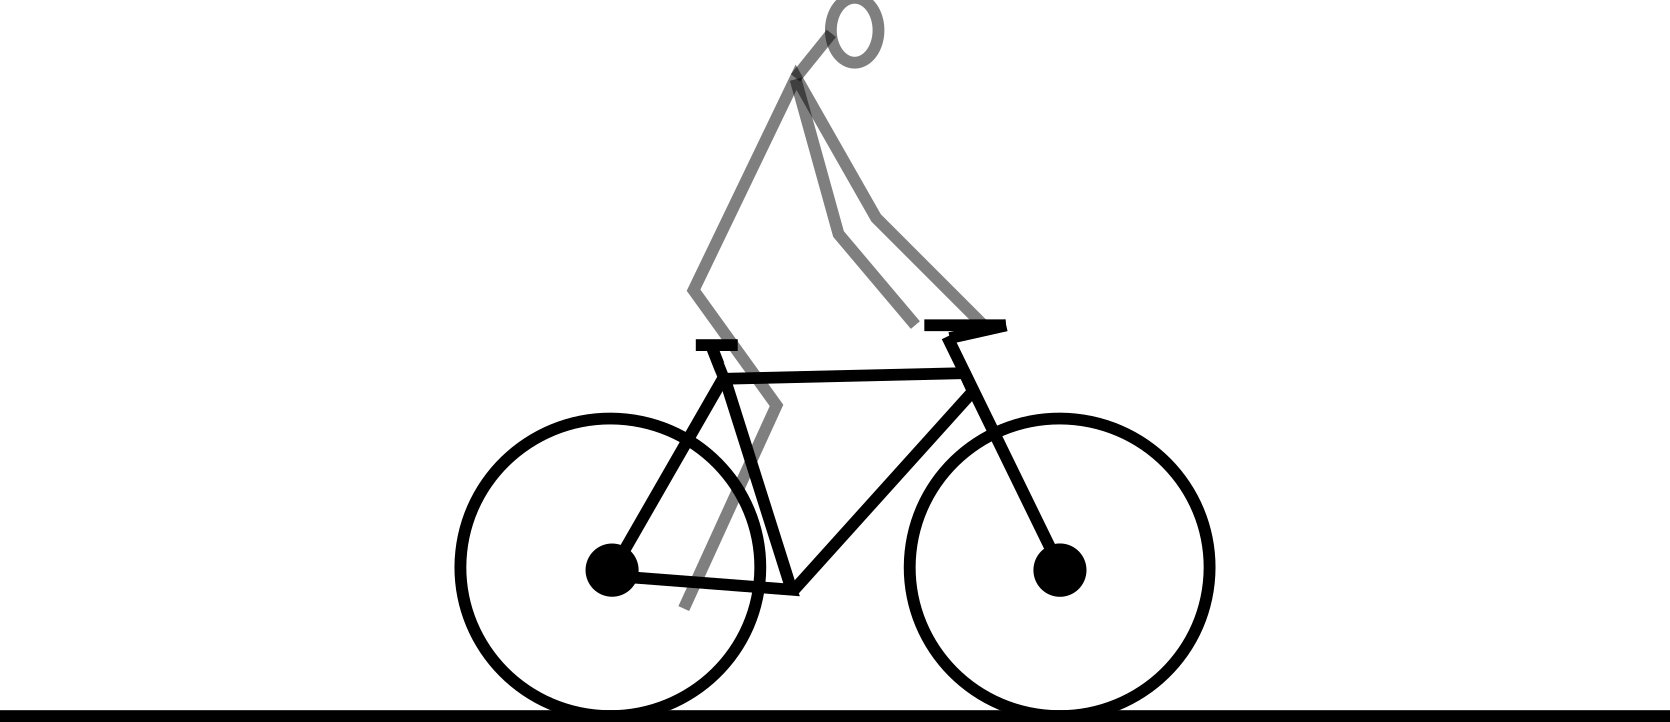
\includegraphics[width=0.9\textwidth]{Images/pitch-over-stage1.png}
        \caption{Normal riding.}
    \end{subfigure}%
    \begin{subfigure}[t]{0.32\textwidth}
        \centering
        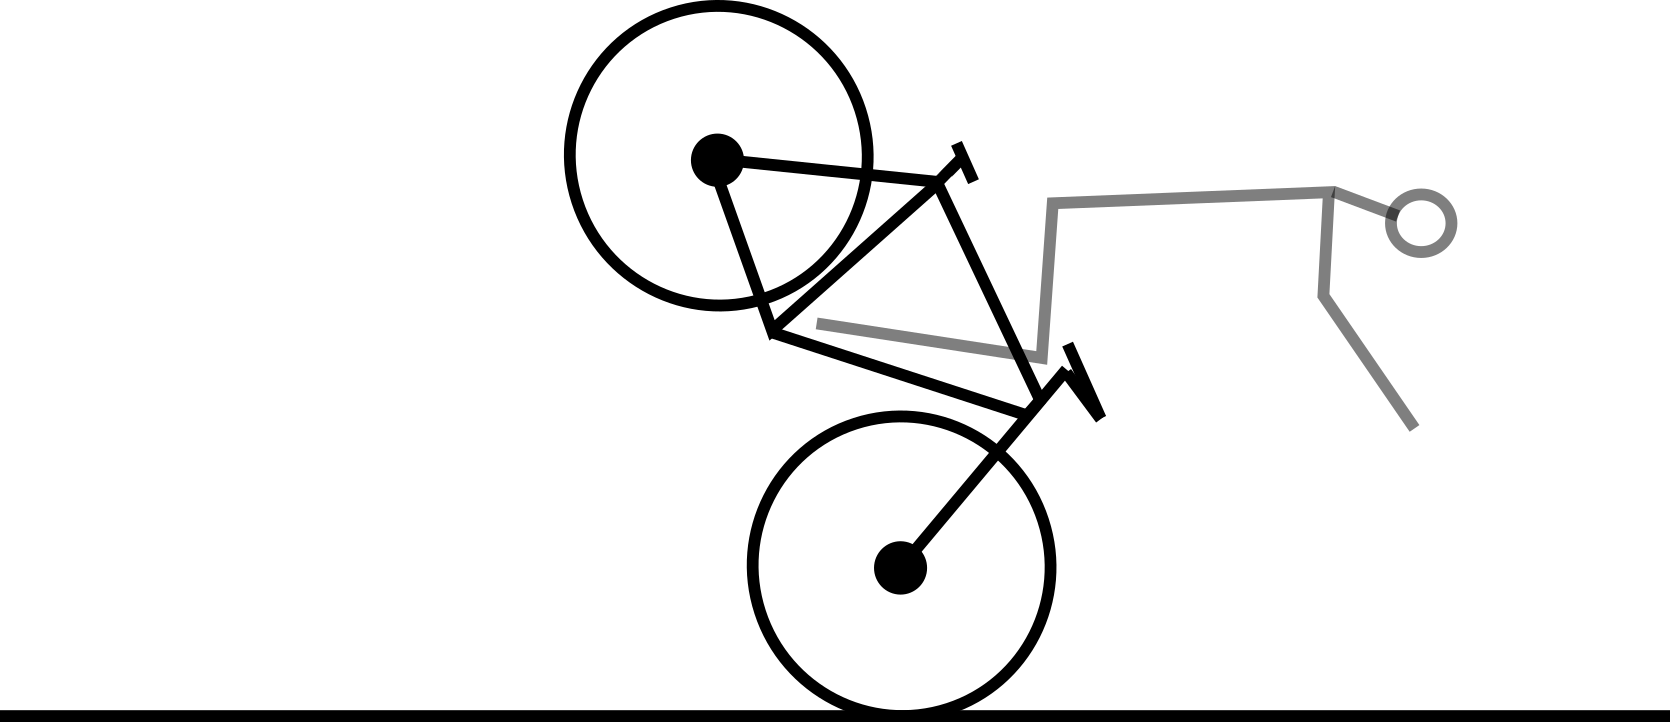
\includegraphics[width=0.9\textwidth]{Images/pitch-over-stage2.png}
        \caption{The rider activates the brakes, and the deceleration generates load transfer that exceeds rear normal force. Therefore, the bicycle exhibits a rotational motion starting around the contact point of the front wheel.}
    \end{subfigure}
    \begin{subfigure}[t]{0.32\textwidth}
        \centering
        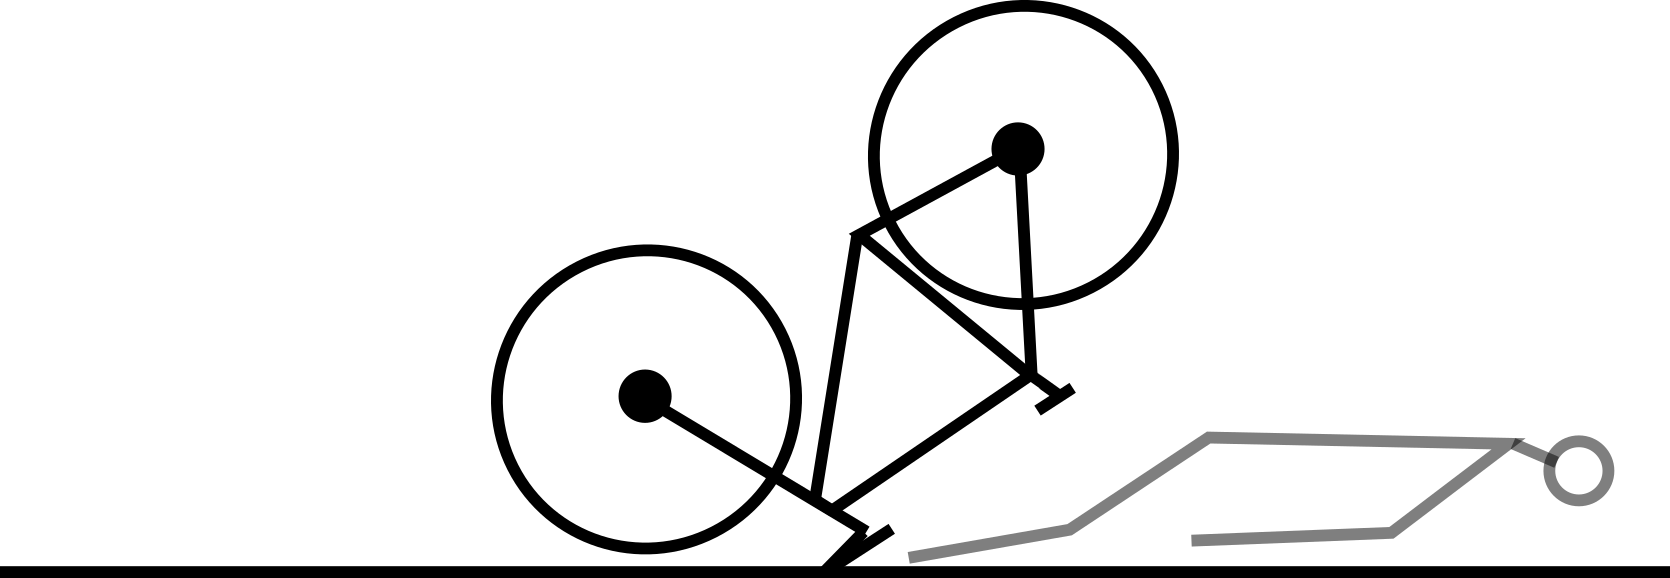
\includegraphics[width=0.9\textwidth]{Images/pitch-over-stage3.png}
        \caption{The rotational inertia of the system produces a complete rotation of the system, which ejects the rider above the handlebar.}
    \end{subfigure}
    \caption{Front pitch-over crash sequence.}
    \label{fig: pitchover}
\end{figure}


When the cause of accidents is assessed as a series of discrete events in a specific time, it is called `Linear chain-of-failure event model' \citep{Lev20}.
%
% These models graphically show the series of events that lead to a crash, however, they often ignore secondary potential factors \citep{Zha22}.
%
% Therefore, towards the aim of `zero fatalities' \citep{Men17}, new models are required, which allow the combination of factors to provide a more integral analysis \citep{Zha22}.
%
Aligned with this idea, we propose a multi-layer sequential classification, which allows to combine the influence of different factors on the outcome of the event.
%
The classification consists of four main layers and three sub-layers, as seen in Figure \ref{fig: flowchart}.
%
The main layers are composed of already known concepts in the field, such as manoeuvres (Table~\ref{tab: manoeuvre}), excitation of the system (Table~\ref{tab: excitation description}), mechanisms of crash (Table~\ref{tab: mechanism description}), and motion of the system during the crash (Table~\ref{tab: motion}).
%
On the other hand, sub-layers expose gaps found in the literature, such as human control in crash or pre-crash scenarios, characteristics of the excitation of the system, and the spatial location of the mechanisms.
%
This is, include information on whether they act on the front or rear wheel, or if the perturbation, if it exists, acts longitudinally, laterally, or vertically on the system.
%
The intention here is not to fill those gaps but to give some cues for future research to address them.
%%


The multi-layer approach allows to classify the crash event with different depth levels according to the available information.
%
Thus, this gives a flexible base that can be applied in different fields, depending on the objective sought.
%%




% Closing paragraph

\subsubsection{Manoeuvre}
%
The first layer consists of the manoeuvre that the rider is executing at the moment of entering the critical scenario, see Table \ref{tab: manoeuvre}.
%
\begin{table}[!h]
\centering
\renewcommand{\arraystretch}{1.3}
\begin{tabularx}{\textwidth}{
  >{\bfseries\raggedright\arraybackslash}p{4cm}
  >{\raggedright\arraybackslash}X
}
\toprule
Manoeuvre & Description \\
\midrule
Longitudinal acceleration & refers to braking and acceleration, both performed by the user \\
Low speed riding & mainly referred to start and stop riding, where users require major balance actions to maintain the bicycle in an upright position. Speed ranges between 0.8 and 2.8 [m/s] \\
Steady and planned cornering & situations where the rider is performing a controlled turn, with a clear trajectory in mind \\
Straight-running & the action of following a straight path, maintaining balance through minor steering adjustments and no major variations on the states of the system \\
Stunting & any action that is not intended for riding, such as riding with one hand, no hands, riding in one wheel, or simply getting on purpose in a challenging-to-control state, which changes and limits the control of the rider on the bicycle \\
\multirow{2}{=}{Unplanned turning/ \\ Avoidance manoeuvre} & the rider executes a sudden evasive turn to avoid an obstacle \\
 & \\[-1.2ex]
\bottomrule
\end{tabularx}
\caption{Types of manoeuvres.}
\label{tab: manoeuvre}
\end{table}



\subsubsection{Excitation of the system}
%
Due to the complexity of the human-bicycle system, it is subjected to several excitations, here collected in three classes.
%
These classes are aligned with \cite{Fel76}, and \citep{Sch12}, where the latter refers to them as direct causes of the crash.
%
Furthermore, a schematic representation of the interplay between the classes is shown in Figure \ref{fig: rider-bike diagram}. 
%
In this work, they are referred as rider, intrinsic, and external, respectively.
%
The description for each of them is given in Table \ref{tab: excitation description}.
%
\begin{table}[h!]
\centering
\renewcommand{\arraystretch}{1.3} % Adjust row height
\begin{tabularx}{\textwidth}{>{\bfseries}lX}
\toprule
Excitation & \textbf{Description} \\
\midrule
Intrinsic & makes reference to any excitation that occurs due to the behaviour of the bicycle itself. This encompasses the modes of vibration and bicycle malfunctions \\
Rider & refers when the major excitation of the system comes from a control action from the rider \\
External & this refers to any perturbation, force, change of state, or influence exerted by the environment on the system \\
\bottomrule
\end{tabularx}
\caption{Types of excitation and their descriptions.}
\label{tab: excitation description}
\end{table}

\begin{figure}[h]
    \centering
    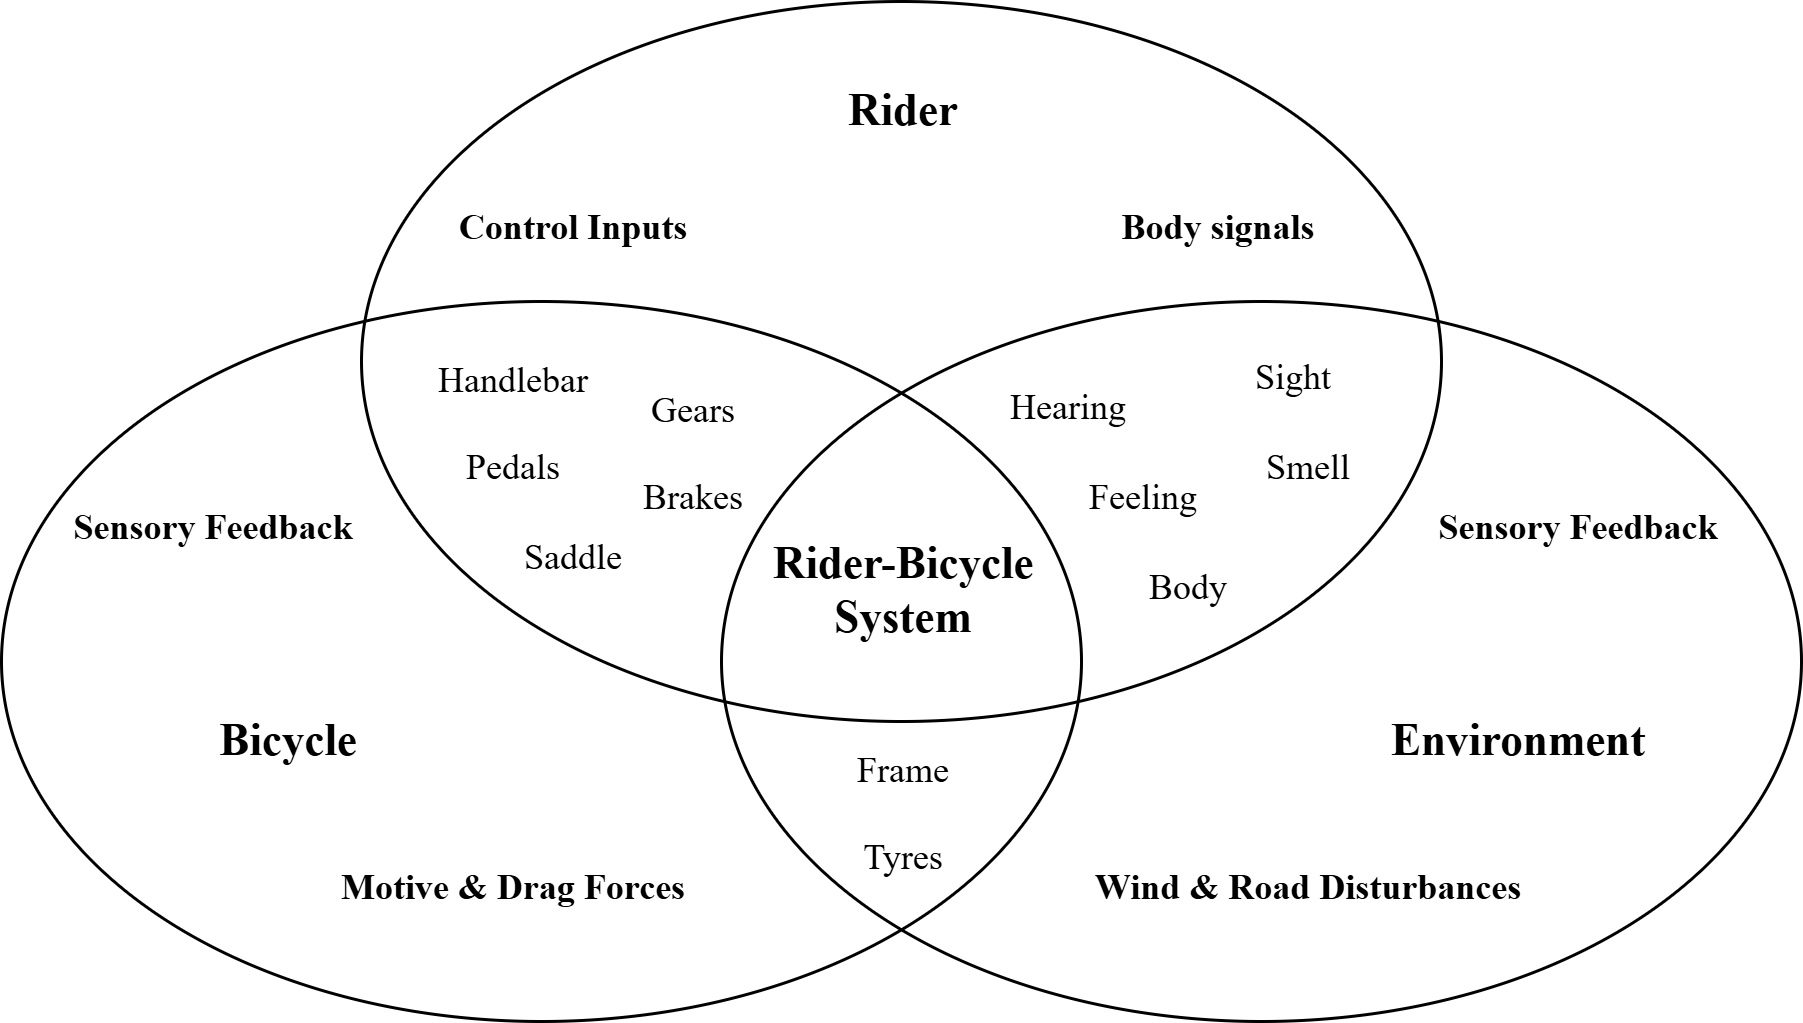
\includegraphics[width=0.75\linewidth]{Images/bicycle-rider-system.png}
    \caption{Rider, bicycle, and environment interfaces and interactions. Adapted from \cite{Lot21}.}
    \label{fig: rider-bike diagram}
\end{figure}



\subsubsection{Mechanisms of crash}
%
In the literature, there are several known mechanisms of crashes, normally clustered as skidding, collisions, falls, among others, as seen in Table \ref{tab: known mechanisms}
%
However, these `boxes' do not fit the broad spectrum of mechanisms, nor capture the dynamics involved in the events.
%
For this reason, we propose the following mechanisms based on the literature, see Table \ref{tab: mechanism description}.
%%
\begin{table}[h!]
\centering
\renewcommand{\arraystretch}{1.3} % Adjust row height
\begin{tabularx}{\textwidth}{
  >{\bfseries\raggedright\arraybackslash}p{4cm}
  >{\raggedright\arraybackslash}X
}
\toprule
Mechanism & Description \\
\midrule
Balance control & this makes reference to the ability of the human to balance the bicycle as an inverted pendulum, moving the steering to control its equilibrium \\
Contact forces & this makes reference to any collision or force exerted on the bicycle, such as collision with an object, or perturbations \\
Load transfer & longitudinal accelerations generate longitudinal load transfer, which remains unnoticed for most casual riders. However, under large accelerations, these load transfer can easily exceed the maximum tolerable values for maintaining the bicycle in a longitudinally stable configuration. Therefore, due to the inertia of the system, a rotational motion is produced, which changes the states of the system out of its boundaries of human control \\
Rider-bicycle joint & the rider interfaces with the bicycle in five points: handlebar (both hands), pedals and saddle. The loss of one or more of these interfaces reduces the control authority \\
Tyre friction & the only constant connection between the bicycle and the environment is on the tyre-ground contact interface. Tyres have a saturation limit for the grip available, when this limit is reached, they start to skid and the rider loses control of the vehicle. Depending on which of the tyres loses grip, the dynamics will change, causing under- or over-steering behaviour \\
\bottomrule
\end{tabularx}
\caption{Crash mechanisms and their descriptions.}
\label{tab: mechanism description}
\end{table}

In the literature, these mechanisms and their approaches are treated as absolutes, with no distinction on the application point.
%
For this reason, we include front or rear, along with longitudinal, lateral or vertical as features to further explain the mechanism.



\subsubsection{Characteristic motion} \label{subsec: crash motion}
%
In the literature, we find three characteristic motions for two-wheeled single-track vehicle crashes \citep{Bed16, Ros17}, see Figures \ref{fig: highside}, \ref{fig: lowside} and \ref{fig: pitchover} for schematic representation of the motions. 
%
Note that motorcycle crash analyses are referenced to explain these crash motions, since the available bicycle-related literature is scarce and does not provide a detailed description, see Table \ref{tab: motion}..
%%

From Section \ref{sec: bike}, we know that crash motions occur directly related to two of the angular degrees of freedom of the rear frame of the bicycle, i.e. pitch and roll.
%
However, due to the unstable nature of bicycle lateral dynamics, roll-related crash motions are sub-divided in three different cases.
%%
\begin{table}[h!]
\centering
\renewcommand{\arraystretch}{1.3} % Adjust row height
\begin{tabularx}{\textwidth}{lX}
\toprule
\textbf{Motion} & \textbf{Description} \\
\midrule
\textbf{Collision ejection} & this sub-class refers to crashes where the final motion is not clear, the main event is a collision that stops the motion of the bicycle, while the rider gets ejected \\
\textbf{Pitch-over} & the main characteristic of this motion is one of the wheels lifting from the ground, following a trajectory that finishes with the front wheel behind the rear wheel \citep{Bec04, Bre10}. Colloquially known as uncontrolled \textit{stoppie} or \textit{wheelie}, depending on whether the motion goes towards the front or the rear, respectively \\
\textbf{Low-side} & the rider-bicycle system follows an excessive roll rate in the same direction as at the beginning. \cite{Cos07} explains it as a yaw movement that causes over-steering rotation \\
\textbf{High-side} & characterised by a skidding motion followed by sudden deceleration of the wheel while in lateral motion, which leads to an extreme negative roll rate with respect to the direction of the initial motion. \cite{Cos07} adds the characteristic of rider upward ejection as a result, frequently occurred in racing motorcycle crashes \\
\textbf{Tip-over} & the bicycle falls into one side as a result of a lack of control at low or no speed. Differs from the low-side crash by the absence of skidding \\
\bottomrule
\end{tabularx}
\caption{Crash motion types.}
\label{tab: motion}
\end{table}

\subsubsection{Unknowns event features}
%
\begin{itemize}
    \item \textbf{Rider factors:} these are intended to explain the interplay between the intrinsic factors of the bicycle and the rider's response.
    %
    Through these factors, the rider understands their own state, senses the environment, and the state of the bicycle.
    %
    It would be interesting to explore how this closed control loop works in critical scenarios.
    \item \textbf{Signal:} this is expected to have a close relation with the triggered mechanism.
    %
    For example, an unstable oscillatory mode of the bicycle would act as a periodic signal, which increases the task demand till the rider loses control.
    \item \textbf{Location:} where the failure mechanism occurs can expose which crash motion is more prone to occur.
    %
    For instance, if the tyre friction mechanism fails at the rear wheel, on the lateral direction, there is a high chance of observe a high-side crash.
\end{itemize}


\subsection{Root causes}
%
The root causes serve as an open field for details about the factors that provide additional information about the crash.
%
These can not be realistically classified in discrete events, since the possibilities are extremely extensive.
%
It is important to note that these are the causes that connect the different layers. 
%
Thus, Table \ref{tab: root causes} provides a brief explanation of how these causality relations should be understood.
%%

\begin{table}[h]
\centering
\renewcommand{\arraystretch}{1.3}
\begin{tabularx}{\textwidth}{
  >{\bfseries\raggedright\arraybackslash}p{3cm}
  >{\raggedright\arraybackslash}X
}
\toprule
Relation & Description \\
\midrule
I--II & how a manoeuvre leads or creates more exposition to one or more of the system's excitations \\
II--III & these are the factors commonly discussed in the literature, such as icy road, aerodynamic perturbations, instabilities, among others \\
III--IV & how one or more mechanisms translate into a crash motion. This causality relation is strongly related to the physics underneath bicycle motion \\
\bottomrule
\end{tabularx}
\caption{Causality relations between layers.}
\label{tab: root causes}
\end{table}


\subsection{Classification diagram}
%
From all the information gathered and explained above, we construct a diagram (cf. Figure \ref{fig: flowchart}) which give cues to follow a descriptive bicycle-crash classification.
%
The diagram shows a sequence of features of an event that lead to a crash; The way of understanding it goes:
%
The rider is executing a manoeuvre, then, the system experiences an excitation that leads to a critical situation.
%
Depending on the human control and the characteristics of the signal, the task demand increases above the boundary of capability of the rider, which causes one or more crash mechanisms to appear.
%
The crash mechanism occur with related spatial information, giving space to the characteristic motions, to finally end in a crash.
%%
%
\begin{landscape}
  \begin{figure}[p]
    \centering
    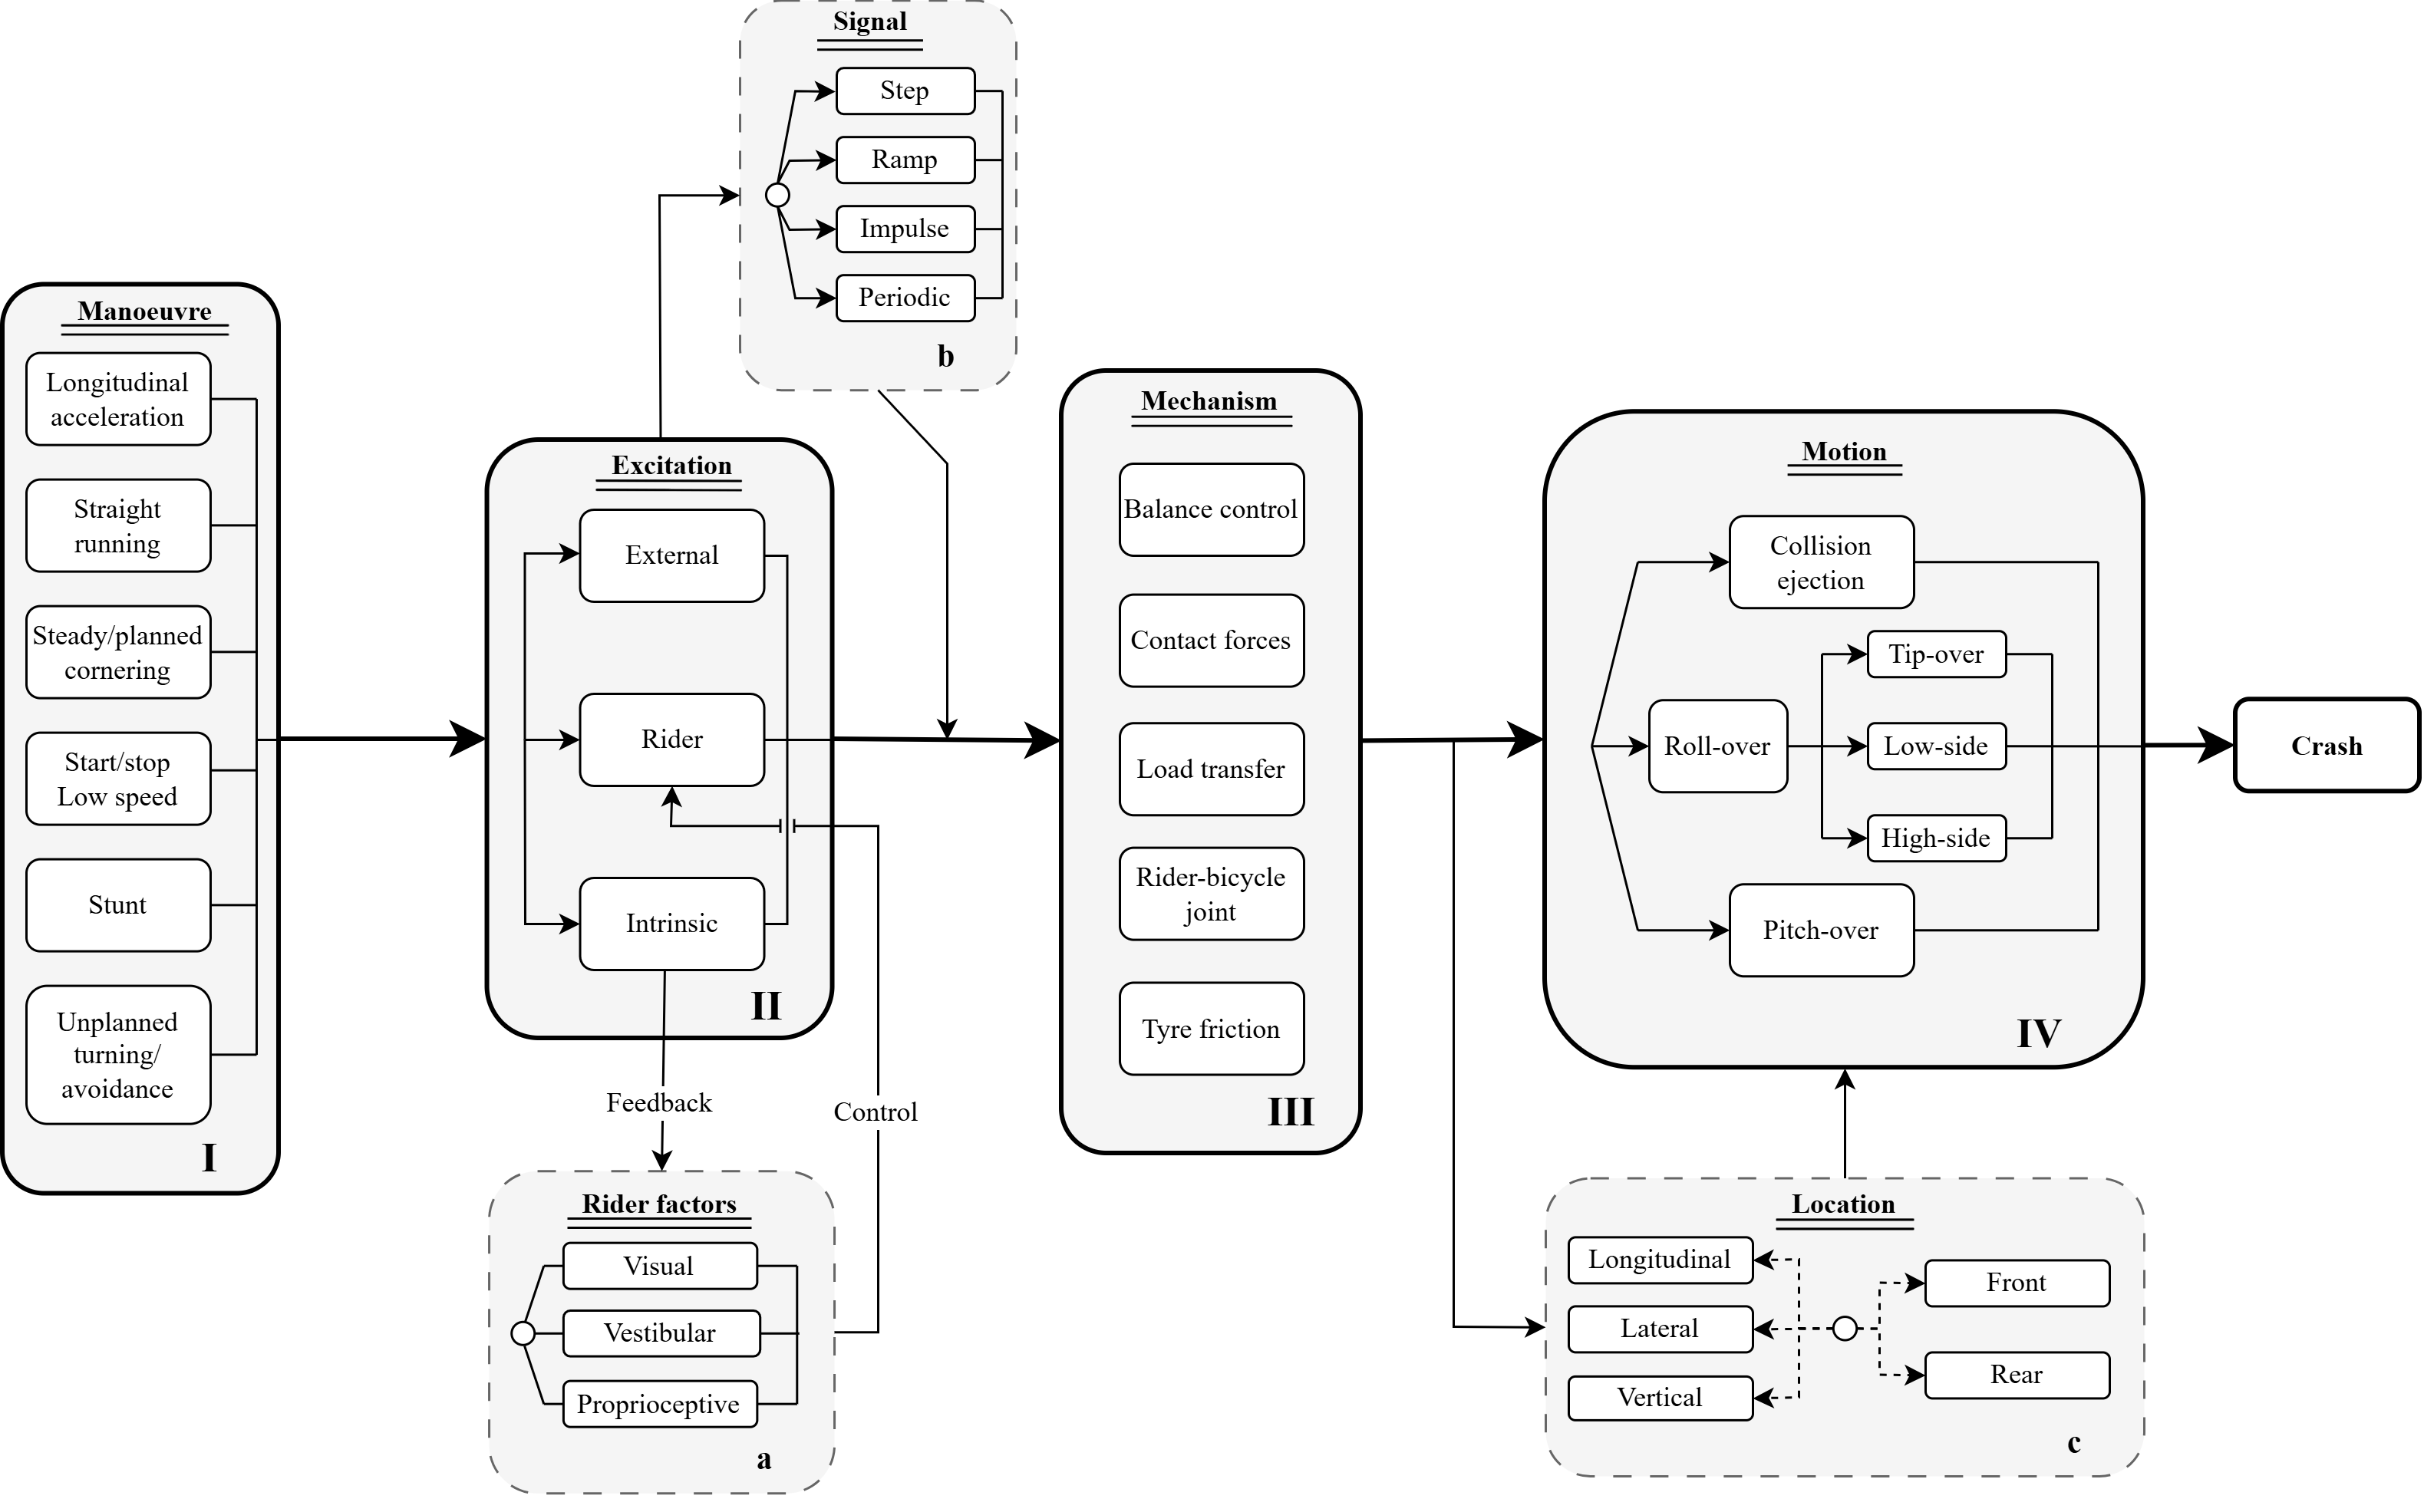
\includegraphics[width=1.5\textwidth, height=\textheight, keepaspectratio]{Images/class-mindmap-v10.png}
    \caption{Multi-layer single-cyclist crash classification. Solid line boxes represent already identified and known concepts in the field. Dashed line boxes represent gaps that are currently not discussed in the literature. Arrows indicate the sequence of the layers. Bold arrows should be understood as `cause'.}
    \label{fig: flowchart}
  \end{figure}
\end{landscape}


For example, Figure \ref{fig: lowside}, the rider is doing a normal-speed turn to the right at $\sim 5$[m/s] (planned cornering).
%
Then, the front wheel steps on a low-grip zone of the road surface (external excitation), which causes the failure mechanism of tyre friction.
%
As the front wheel loses grip, the rotational dynamics change and it produces an understeering behaviour, from which the rider can not retake control of the balance through steering inputs, leading to an excessive roll rate (low-side crash).
%
Here, would be interesting to know what is the available time between grip decrease and the first response from the rider, or how the loss of grip acts on the system as a signal.
%%

\section{Discussion} \label{sec: discussion}
%
In this work, we reviewed the literature where single-cyclist crash classifications, factors, and mechanisms are discussed.
%
We found a gap in how existing classifications capture the dynamics of the bicycle and its interaction with the environment.
%
In addition, many commonly used terms are not clarified in all studies.
%
Therefore, we presented the key concepts used in this work, reviewed the existing information and proposed a new classification.
%%


% Bicycle dynamics
Based on bicycle dynamics theory, we were able to capture the possible failure mechanisms that lead to crashes.
%
Particularly, we highlight the unstable modes of vibration as a mechanism that overcomes the control capability of the rider.
%
Similarly, assessing the tyre-ground friction as a general concept encompasses the crashes due to slippery surfaces and road irregularities.
%
Moreover, this mechanism explains the cases where cyclists veers off the road during a corner due to reaching the maximum available friction.
%%


% Contrast with existing classifications

The main categories used for the nature of the excitation are in agreement with \cite{Fel76} and \cite{Sch12}. 
%
However, on the sub-categories of causes, here referred as mechanisms, we find major differences with respect to \cite{Sch12}.
%
Although there are some similarities, such as identifying collisions, braking mistakes, bicycle malfunction or steering disturbances, the first difference comes from the use of combinations of different mechanisms to explain a single event.
%
With this method, we rank the mechanisms identified according to their hypothesised share of the outcome.
%%


Although \cite{Sch12} took into account the dynamics of the bicycle in his work, these factors do not accurately capture the mechanisms that occur.
%
In general, we find categories narrowed to specific events, which show the effects of infrastructure failures.
%
Indeed, Schepers' work did not aim to capture enough information to reconstruct the event, but an attempt to standardise single-cyclist crashes.
%
However, the information obtained is scarce if the interest is on recreating a certain crash scenario, missing the intended manoeuvre by the rider, or the motion of the system during the crash.
%%


Alternatively, \cite{Gil21a} includes the fall type in his classification.
%
Compared to Gildea's classification, we agree on the pitch-over and roll-over motions, subdividing the latter into three specific crash motions.
%
However, the fall motion presented as `skid-out' may represent a skidding mechanism under large lateral loads, which results in a crash by colliding with the kerb or running off the road.
%
Therefore, we differ in defining skidding as a crash motion, since it can be explained as a primary mechanism, which results in a low-side roll-over motion.



\subsection{Mechanisms}
%
One important part of the present work is providing a detailed description of the hypothesised crash mechanisms.
%
From the mechanisms present in this classification, only `tyre friction' and `contact forces' are explicitly discussed in the literature \citep{Alg22, Bec16, Boe17, Her18, Sch12}.
%
However, authors prefer a broader approach where similar mechanisms belong to the same class, e.g. skidding on wet, icy or leaf-covered pavement, all of them represent a loss of tyre friction.
%
Furthermore, crashes involving collision with objects, temporal or permanent, are clustered as contact forces, which also applies for wheels getting stuck on tram tracks.
%
Similarly, low-speed `loss of control' crashes are explained through lateral and longitudinal balance control mechanisms.
%%


Based on the crash model from \cite{Ful05}, describing a crash mechanism as `loss of control' becomes redundant, since all crashes occur due to loss of control.
%
Therefore, is it aimed to avoid classes that are not descriptive of the event, such as `other', `unknown' or `loss of control'.
%%


The new proposed mechanisms are related to the known mechanisms as shown in Table \ref{tab: mechanism relation}

\scriptsize
\begin{table}[!h]
    \centering
    \begin{tabular}{ l c c c c c c }
    \toprule
    \textbf{Mechanism} & 
    \makecell{\textbf{Balance}\\\textbf{control}} & 
    \makecell{\textbf{Contact}\\\textbf{forces}} & 
    \makecell{\textbf{Load}\\\textbf{transfer}} & 
    \makecell{\textbf{Rider}\\\textbf{bicycle joint}} & 
    \makecell{\textbf{Tyre}\\\textbf{friction}} \\
    \midrule
    Braking mistakes              & ~ &   & \textbullet & ~ & \textbullet \\ 
    Caught in track               & \textbullet & \textbullet & ~ & ~ & ~ \\ 
    Collision                     & ~ & \textbullet & ~ & ~ & ~ \\ 
    Crossing a threshold          & ~ & \textbullet & \textbullet & ~ & \textbullet \\ 
    Evasive manoeuvre             & \textbullet &   & \textbullet & ~ & ~ \\ 
    Fall                          & \textbullet &   & ~ &  ~ & ~ \\ 
    Front wheel hit               & \textbullet & \textbullet & ~ & ~ & ~ \\ 
    Getting on off the bike       & \textbullet &   & ~ & ~ & ~ \\ 
    Kerb hit                      & \textbullet & \textbullet & ~ & ~ & ~ \\ 
    Loss of control on a descent  & \textbullet &   & \textbullet & ~ & ~ \\ 
    Low speed loss of balance     & \textbullet &   & ~ & ~ & ~ & ~ \\ 
    Mechanical malfunction        & \textbullet &   & ~ & \textbullet & ~ \\ 
    Object on the road            & ~ & \textbullet & ~ & ~ & ~ \\ 
    Riding off the road           & ~ & \textbullet & ~ & ~ & \textbullet \\ 
    Road surface condition        & ~ &   & ~ & ~ & \textbullet \\ 
    Skidding                      & ~ &   & ~ & ~ & \textbullet \\ 
    Slipping off the pedals       & ~ &   & ~ & \textbullet & ~ \\ 
    Something caught on the wheel & ~ &   & \textbullet & ~ & ~ \\ 
    Striking pothole              & ~ & \textbullet & ~ & ~ & \textbullet \\ 
    Stunt                         & \textbullet &   & \textbullet & \textbullet & ~ \\ 
    Tram track interaction        & \textbullet & \textbullet & ~ & ~ & \textbullet \\ 
    Turning mistake               & \textbullet &   & ~ & ~ & ~ \\ 
    Unable to keep balance        & \textbullet &   & ~ & ~ & ~ \\ 
    Uneven road                   & ~ &   & ~ & ~ & \textbullet \\ 
    \bottomrule
    \end{tabular}
    \caption{Relation between proposed and known mechanisms.}
    \label{tab: mechanism relation}
\end{table}
\normalsize



\subsection{Questionnaire results}
%
The questionnaire, designed to evaluate the scope of this study, revealed a high level of agreement regarding detected mechanisms and motions.
%
However, the remaining disagreement may be explained by the statement \textit{`Crash cause is similar to beauty: it is in the eye of the beholder'} \citep{Shi19}.
%
Shinar’s work highlights that crash analysis varies among authors depending on their primary focus.
%
His findings indicate that police analyses often attribute crashes to operator error, reflecting their emphasis on law enforcement.
%
Conversely, road engineers frequently conclude that roadway defects contribute to approximately 76\% of crashes.
%
Thus, classification and interpretation are strongly influenced by the study’s objectives and the perspective of the analyst.
%%


Based on responses from ten participants, the classification model was expanded to include \textit{collision ejection} and \textit{tip-over} within the crash motion layer.
%
Furthermore, agreement exceeded 75\% for manoeuvre, system excitation, and crash motion categories when compared to the author’s responses.
%
In contrast, agreement on mechanisms decreased to 50\%, likely due to Shinar’s hypothesis and the limited quality of available video data.
%
Finally, among the 100 classified videos, the only open-field response was in the `other excitation' question, suggesting that the proposed classification adequately captured all observed events.
%%


\subsection{Crash types}
%
Since the most prominent characteristic of a crash is the motion, the ways of crashing are named after them, and the hypothesised mechanisms come as an additional description for the event.
%
In general, the authors recommend calling crashes in a descriptive way, following a reverse order from Figure \ref{fig: flowchart}.
%
Thus, the general structure would look like: `motion' due to `mechanism-root cause', as a result of `excitation' when `manoeuvre'.
%
In this way, most low-speed crashes will be a tip-over, due to balance control issues.
%
Similarly, cornering crashes are mainly low-side crashes, due to tyre friction issues, where the root cause will be commonly detailed.
%
At last, an example is \textit{`...he had a low-side crash due to grip issues on an icy road, as a result of an external excitation when he was doing a turn to the right'} (Figure \ref{fig: lowside}).
%%


\subsection{Limitations and future work}
%
The limitations of this work are related to the available data used to test the classification, since only videos from social media were used, without personal assessment of the subjects.
%
It is expected that the available videos are biased towards the level of visual impact that they provoke.
%
In addition, the possible root causes for the mechanisms are no further discussed since they are out of the scope of this work.


For future work, it is strongly recommended to perform experiments on critical scenarios to prove the hypothesised mechanisms against empirical results.
%




% Added value

Altogether, this work contributes to the state of the art by providing a description of commonly used concepts that are not properly defined in current articles in the field.
%
Additionally, we formulate a multi-layer classification that provides more information about the crashes and clusters them according to similar dynamic characteristics.
%
Moreover, this work highlights the necessity of human motion and control data to further understand the role of the rider in critical scenarios.
%%

\section{Conclusion}
%
In summary, this study reviewed existing literature on single-cyclist crashes, identifying various classification methods and mechanisms, none of which explicitly addressed bicycle dynamics.
%
To bridge this gap, bicycle dynamics theory was examined to explain known mechanisms and provide a more rigorous theoretical foundation.
%
Based on these insights, a multi-layer classification that integrates established knowledge while addressing existing gaps in the field was proposed.
%
Despite these efforts, classifying bicycle crashes remains challenging due to incomplete information and the influence of study objectives on interpretation.
%
Moreover, even with linear event descriptions, multiple interacting factors shape the outcome of critical scenarios.
%
Finally, a significant knowledge gap persists regarding human responses to specific signals within a system under pre-crash conditions.




\section*{Acknowledgement}
%
Funding: This project has been made possible in part by grant number 2022-252796 from the Chan Zuckerberg Initiative DAF, an advised fund of Silicon Valley Community Foundation.

% \section*{Declaration of generative AI and AI-assisted technologies in the writing process}

% During the preparation of this work the authors used Grammarly in order to revise the writing in the text. After using this tool/service, the authors reviewed and edited the content as needed and takes full responsibility for the content of the published article.

\section*{CRediT}

\textbf{Benjamín González:} Investigation, writing - original draft, 
%
\textbf{Ajay Seth:} Supervision,
%
\textbf{Alfred Schouten:} Supervision,
%
\textbf{Jason K. Moore:} Supervision.

% https://www-elsevier-com.tudelft.idm.oclc.org/researcher/author/policies-and-guidelines/credit-author-statement


\small
\bibliography{Benjamin-Reads.bib}

% \section*{Appendix}


\end{document}
